


\section{Amplification de l'effet photoélectrique par le chlore}

Le chlore est une espèce souvent négligé dans les réseaux d'astrochimie en raison de sa faible abondance dans les PDR (voir \ref{tab:gaz}). Pourtant, des espèces dérivées du chlore telles que $\mathrm{H}_2\mathrm{Cl}^+$,HCl et $\mathrm{HCl}^+$ ont été observées par Herschel dans plusieurs sources de la Galaxie et notamment dans le nuage moléculaire de la barre d'Orion \cite{Neufeld2012,Neufire2009, Schilke}. Ses propriétés chimiques sont connues et étudiées par \cite{Neufire2009,Amin,Schilke} et l'équipe de Meudon avait brièvement commencé à observer les effets du chlore dans le code PDR. Ils avaient constaté que le chlore rendait le gaz plus chaud en bord atomique de nuage mais qu'il causait également des irrégularités dans les profils de densités et de température, pouvant traduire soit un problème numérique soit un nouvel effet dans les PDR. A l'occasion du stage qui traite explicitement des processus thermiques dans les nuages interstellaires, nous avons étudié les conséquences du chlore dans le code PDR.


\begin{table}[!h]
    \centering
    \begin{tabular}{|l|c|c|}
    \hline
     X & $\delta_X$ & $\mathrm{PI}\ (eV)$   \\
     \hline
     H    &  $1$          &     13.6   \\
     He   &  $0.1$        &    24.6      \\
     O    &  $3.2\,10^{-4}$ &    13.6    \\
     C    &  $1.3\,10^{-4}$ &    11.3    \\
     Ne   &  $6.9\,10^{-5}$ &    21.6    \\
     N    &  $4.5\,10^{-5}$ &    14.5    \\
     S    &  $1.9\,10^{-5}$ &    10.4    \\
     Ar   &  $3.3\,10^{-6}$ &    15.8    \\
     Si   &  $8.2\,10^{-7}$ &    8.2    \\
     \color{red}Cl  &  \color{red}$1.8\,10^{-7}$ &    \color{red}13    \\
     F    &  $1.8\,10^{-8}$ &    17.4    \\
     Fe   &  $1.5\,10^{-8}$ &    7.9    \\
     \hline
    \end{tabular}
    \caption{Abondances élémentaires dans le gaz}
    \begin{minipage}{\textwidth}
    La fraction élémentaire $\delta_X$ est le rapport de la densité de l'espèce $X$ par la densité d'élément hydrogène dans le gaz. $\mathrm{PI}$ est le potentiel de ionisation de l'espèce en électron volt.
    \end{minipage}
    \label{tab:gaz}
\end{table}{}

% \begin{figure}[!htbp]
%     \centering
%     \begin{subfigure}[t]{0.49\textwidth} % "0.49" donne ici la largeur de l'image
%         \centering 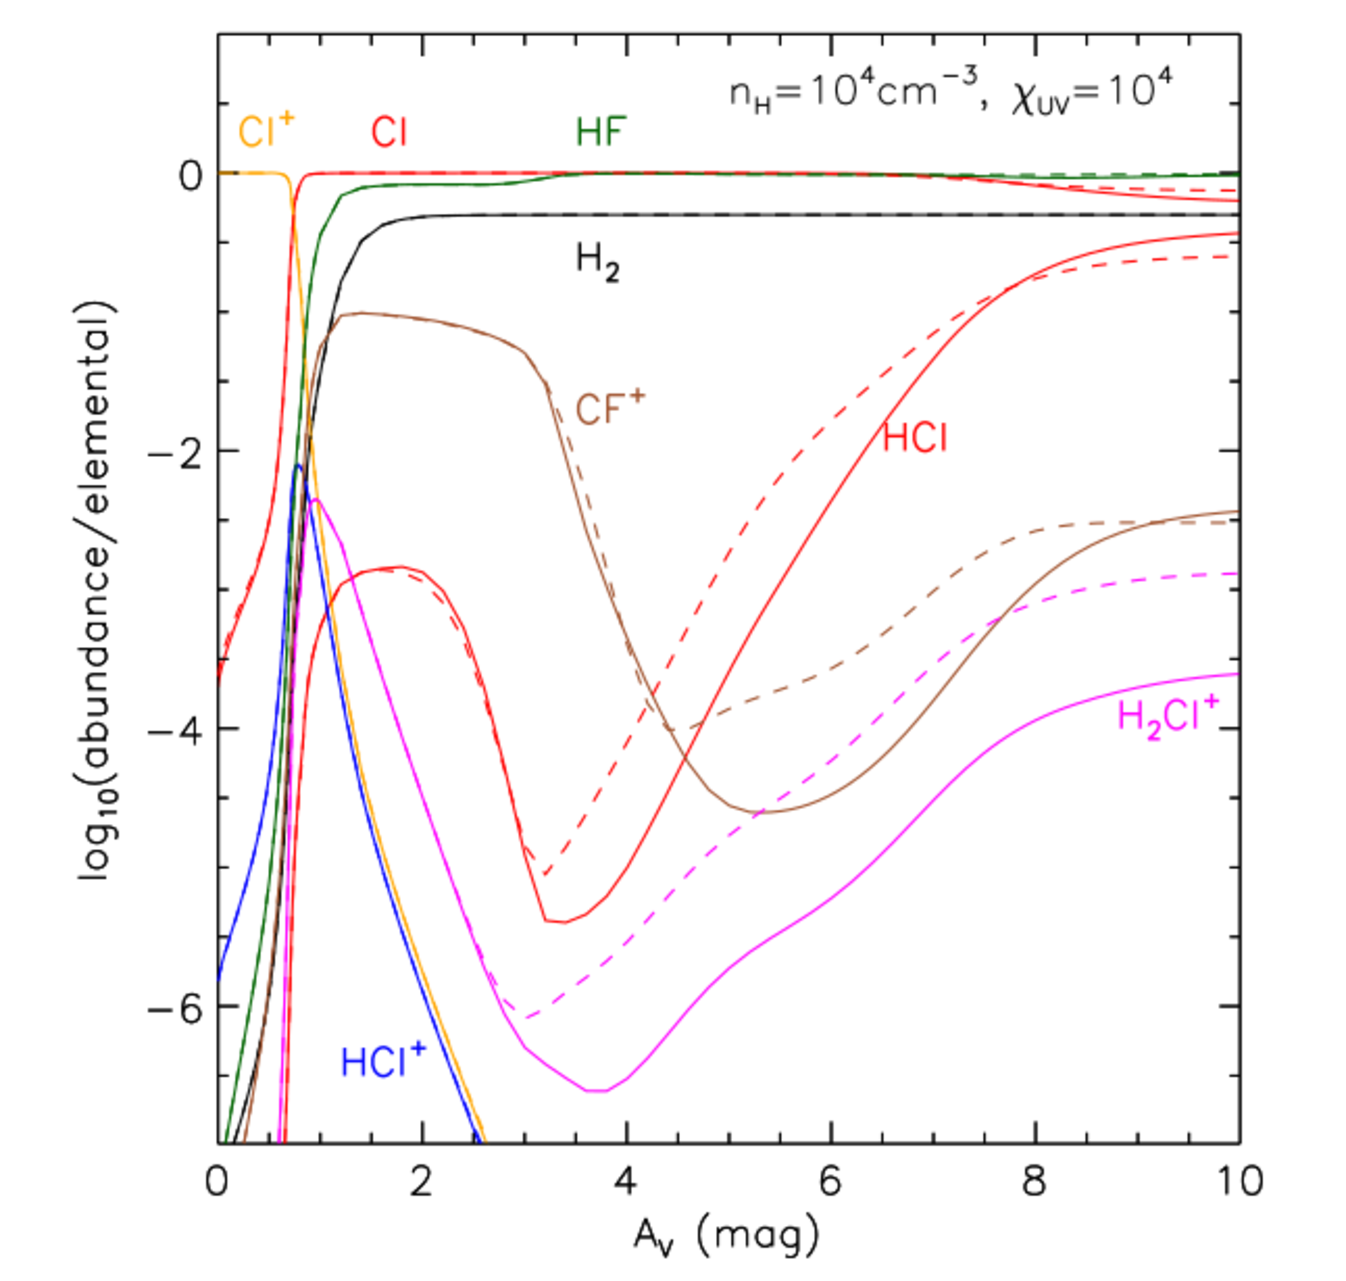
\includegraphics[trim = {0 0 0 0cm},clip,width=1\textwidth]{figure/Cl/neufire/dens.pdf}
%         \caption{}
%     \end{subfigure}
%     ~ 
%     \begin{subfigure}[t]{0.49\textwidth}
%         \centering 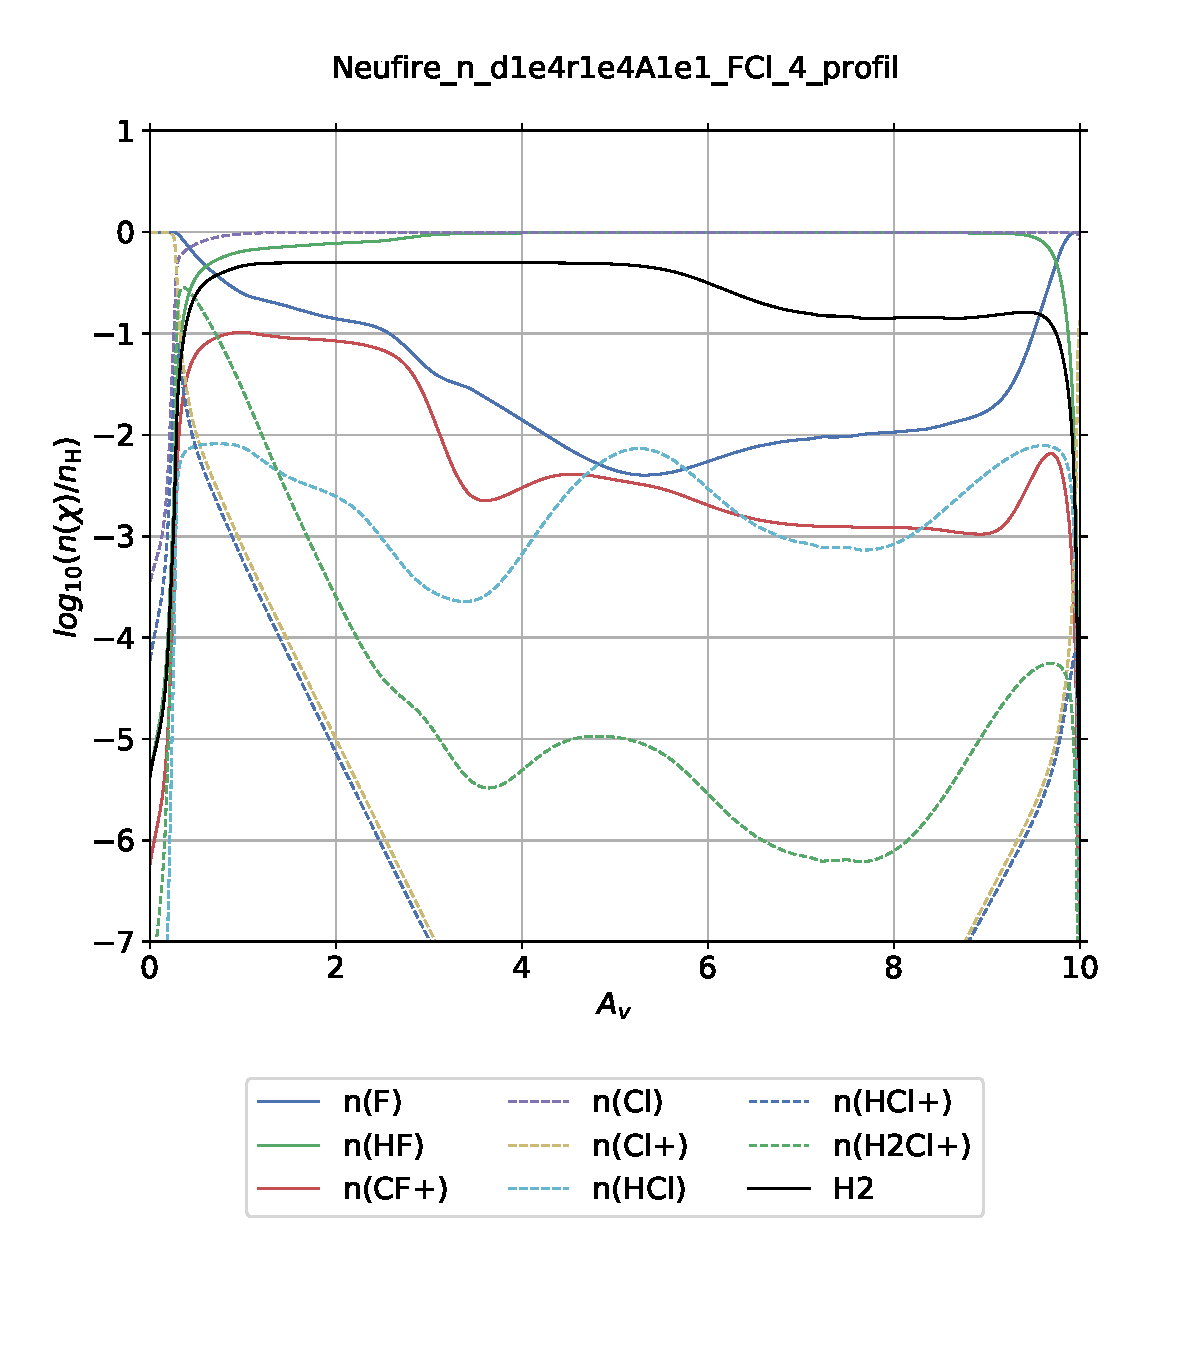
\includegraphics[trim = {0 2cm 0 1.8cm},clip,width=1\textwidth]{figure/Cl/neufire/HCl_profil.pdf}
%         \caption{}
%     \end{subfigure}
    
%     \caption{Profil de densité pour un modèle isochore $n_\mathrm{H} = 10^4 \mathrm{cm}^{-3}$ et $\chi_\mathrm{UV} = 10^4$. La figure de gauche (a) est extraite de \cite{Neufire2009} où les profils sont obtenus à partir d'une version modifié du code de \cite{Kaufman2006}. Le trait plein est un calcul avec un taux de ionisation par les rayons cosmiques de $1.8 \times 10^{−17 } \mathrm{s}^{-1}$ par atome d'hydrogène, tandis qu'en pointillé $1.8 \times 10^{−16} \mathrm{s}^{-1}$ . A droite (b) le code PDR de Meudon résout la PDR en utilisant le même réseau chimique proposé dans l'article.}
%     \label{fig:Cl:neufire}
% \end{figure}



\subsection{Comparaison de profil de température}

Afin de tester l'impact du chlore, on a résolu à l'aide du code PDR deux modèles à des conditions typiques de nuage ($n_{\mathrm{H}} = 10^5\ \mathr{cm}^{-3}$, $\chi = 10^4$), l'un sans chlore et l'autre l'incluant (figure \ref{fig:ClT}). On retrouve le résultat précédent que le bord atomique du nuage est plus chaud de $1000$ K. % et que le profil de température est discontinue aux alentours de $A_\mathrm{v} \sim \, \mathrm{mag}$. 
Pour comprendre l'origine de cette augmentation de température on a tracé les taux de chauffage et de refroidissement en fonction de la température au bord du nuage (figure \ref{fig:ClHC}). %(à $A_{\mathrm{v}} = 10^{-6}\,\mathrm{mag}$). 
L'équilibre thermique du gaz est déterminé par l'intersection des courbes de chauffage et de refroidissement. On voit, en effet, qu'ajouter du chlore dans le code PDR, augmente la courbe de chauffage (en trait plein) à partir de $T\geq 1000$ K et repousse le point d'intersection vers des températures plus chaudes. Pour ces conditions physiques de PDR, le bord de nuage est principalement chauffé par le pompage UV de $\mathrm{H}_2$ et par l'effet photoélectrique sur les grains tandis qu'il est refroidit par les émissions des raies de $\mathrm{O}$ et du $\mathrm{C}^+$. A la vu de la figure \ref{fig:ClHC}, on en conclut que l'augmentation du chauffage total du gaz est causé par celle de l'effet photoélectrique qui est représenté en pointillé. \newline 

L'allure du taux de l'effet photoélectrique indique l'existence une possible bistabilité thermique en bord atomique de nuage, soit que les courbes se coupent en trois températures d'équilibres dont deux sont stables et une instable. Une température d'équilibre est instable si une perturbation la déplace de son point d'équilibre, c'est à dire qu'une perturbation positive de température rend le taux de chauffage plus grand que le taux de refroidissement. Ceux de la figure \ref{fig:ClHC} sont stables car si l'on refroidit le gaz alors le chauffage devient plus intense ce qui ramène le gaz à la température d'équilibre. \newline 


\begin{figure}[!h]
    \centering
    \begin{subfigure}[t]{0.45\textwidth} % "0.45" donne ici la largeur de l'image
        \centering 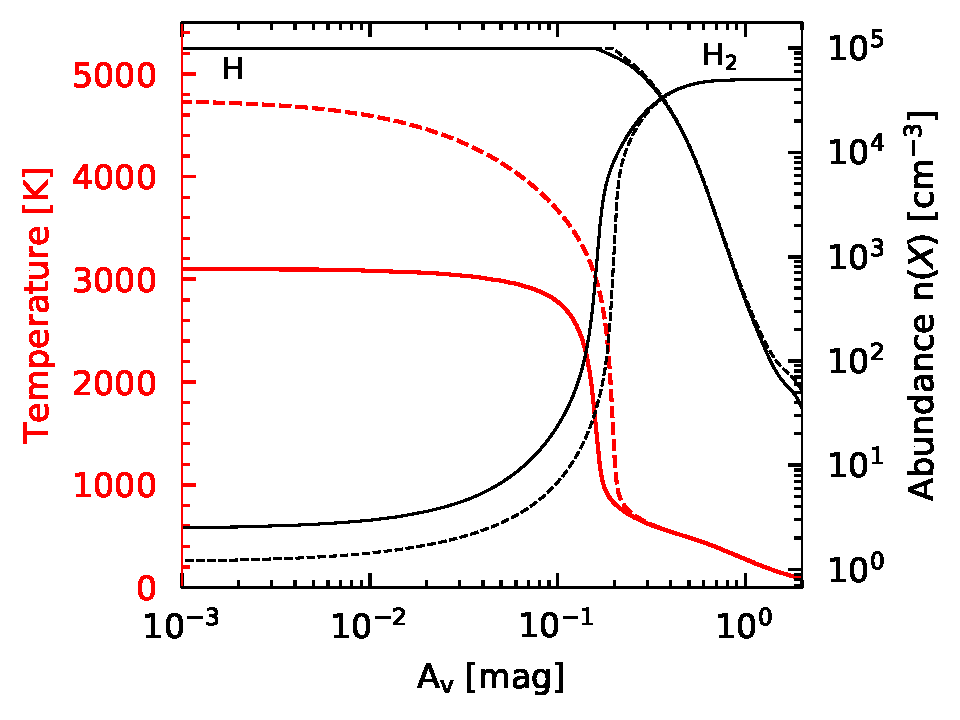
\includegraphics[trim = {0 0 0 0cm},clip,width=1\textwidth]{figure/Cl/profilT.pdf}
        \caption{Profil de température et densité en fonction de la profondeur dans le nuage}\label{fig:ClT}
    \end{subfigure}
    ~ 
    \begin{subfigure}[t]{0.45\textwidth}
        \centering 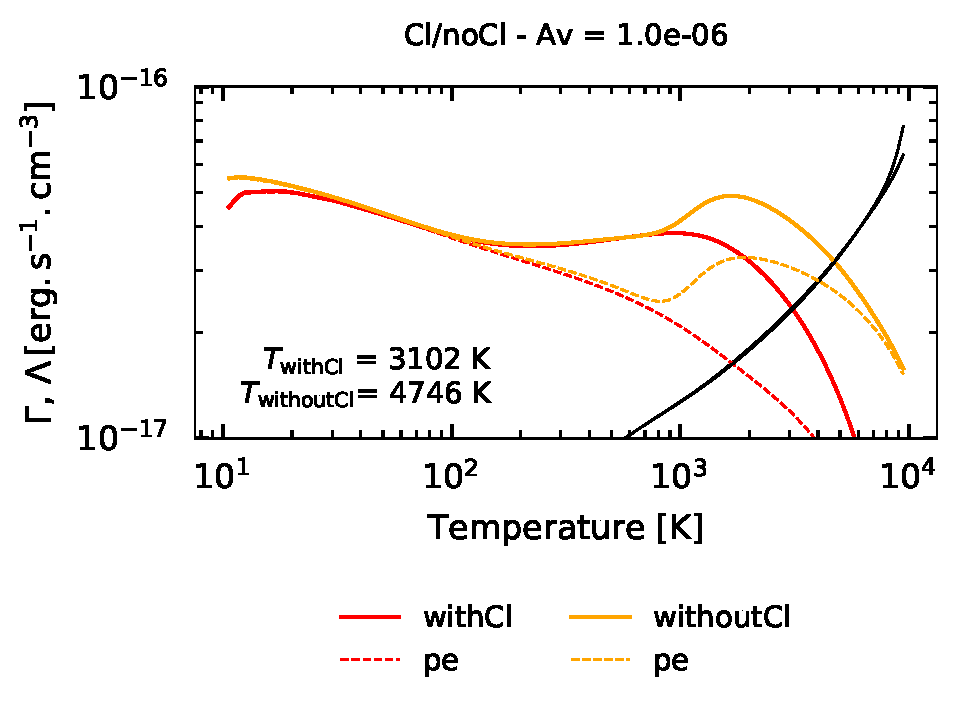
\includegraphics[trim = {0 0 0 1cm},clip,width=1\textwidth]{figure/Cl/GCcomp_h_1p0em06.pdf}
        \caption{Taux de chauffage et refroidissement en fonction de la température du gaz au bord atomique du nuage ($A_{\mathrm{v}} = 10^{-6}$)}\label{fig:ClHC}
    \end{subfigure}
    \caption{Impact du chlore sur les profils - modèles à densité constante ($n_{\mathrm{H}} = 10^5\ cm^{-3}$, $\chi = 10^4$)}
    \begin{minipage}{\textwidth}
    Sur la figure (a) la température est tracé en rouge tandis que les densités de $\mathrm{H}$ et $\mathrm{H}_2$ sont en noir. Le trait plein est le modèle sans chlore tandis les pointillés est le modèle contenant du chlore. Pour la figure (b), les traits pleins en rouge et orange représentent les taux de chauffage total qui sont la somme du chauffage par pompage UV de $\mathrm{H}_2$ et de l'effet photoélectrique sur les grains. Comme l'on s'intéresse particulièrement à l'effet du chlore sur l'effet photoélectrique, celui ci est représenté en pointillé. Les courbes en noires sont les taux de refroidissement total des deux modèles. Ils ne varient pas ou à peine selon que l'on ajoute du chlore ou non.
    \end{minipage}
\end{figure}


\subsection{Rôle du chlore}

Il faut maintenant comprendre l'origine de l'augmentation de l'effet photoélectrique à $T\geq 1000$ K  et chercher dans quelles conditions physiques de PDR, l'instabilité thermique peut avoir lieu. En isolant les réactions chimiques principales et en considérant les processus thermiques dominants, on a construit un modèle semi-analytique permettant d'explorer l'espace des paramètres des PDR et de déterminer les conditions où l'instabilité peut avoir lieu. \newline 

On a étudié les réactions chimiques principales qui se déroulent en bord de nuage atomique et démontré que le chlore joue le rôle de catalyseur de l'effet photoélectrique. Le mécanisme est illustré sur la \autoref{fig:catalyseur}.
Le champs de rayonnement UV, intense en bord de nuage atomique, photoionise le chlore et produit des ions $\mathrm{Cl}^+$ et des électrons. Le transfert de charge du $\mathrm{Cl}^+$ avec l'hydrogène est une réaction rapide qui permet au chlore de se rendre de nouveau disponible pour la photoionisation. Le chlore permet ainsi de ioniser indirectement l'hydrogène. Par conséquent, la fraction électronique du gaz augmente.  \newline 

Or on sait que l'effet photoélectrique sur les grains fonctionne d'autant plus que la fraction électronique dans le nuage est importante \footnote{Une forte densité d'électrons rend plus facile la recombinaison électronique des grains ce qui maintient le degré d'ionisation des grains raisonnablement faible. Il est plus facile d'arracher un électron d'un grain neutre que d'un grain qui a déjà été ionisé.}. 
L'effet photoélectrique chauffe ainsi le gaz ce qui améliore l'efficacité du transfert de charge du $\mathrm{Cl}^+$ avec l'hydrogène. 
En d'autres termes, le chlore induit une rétroaction positive de l'effet photoélectrique sur les grains. Cet emballement a tendance à chauffer le gaz à des températures nettement plus fortes et ce malgré la faible abondance du chlore. \newline

\begin{figure}[!h]
   \centering
        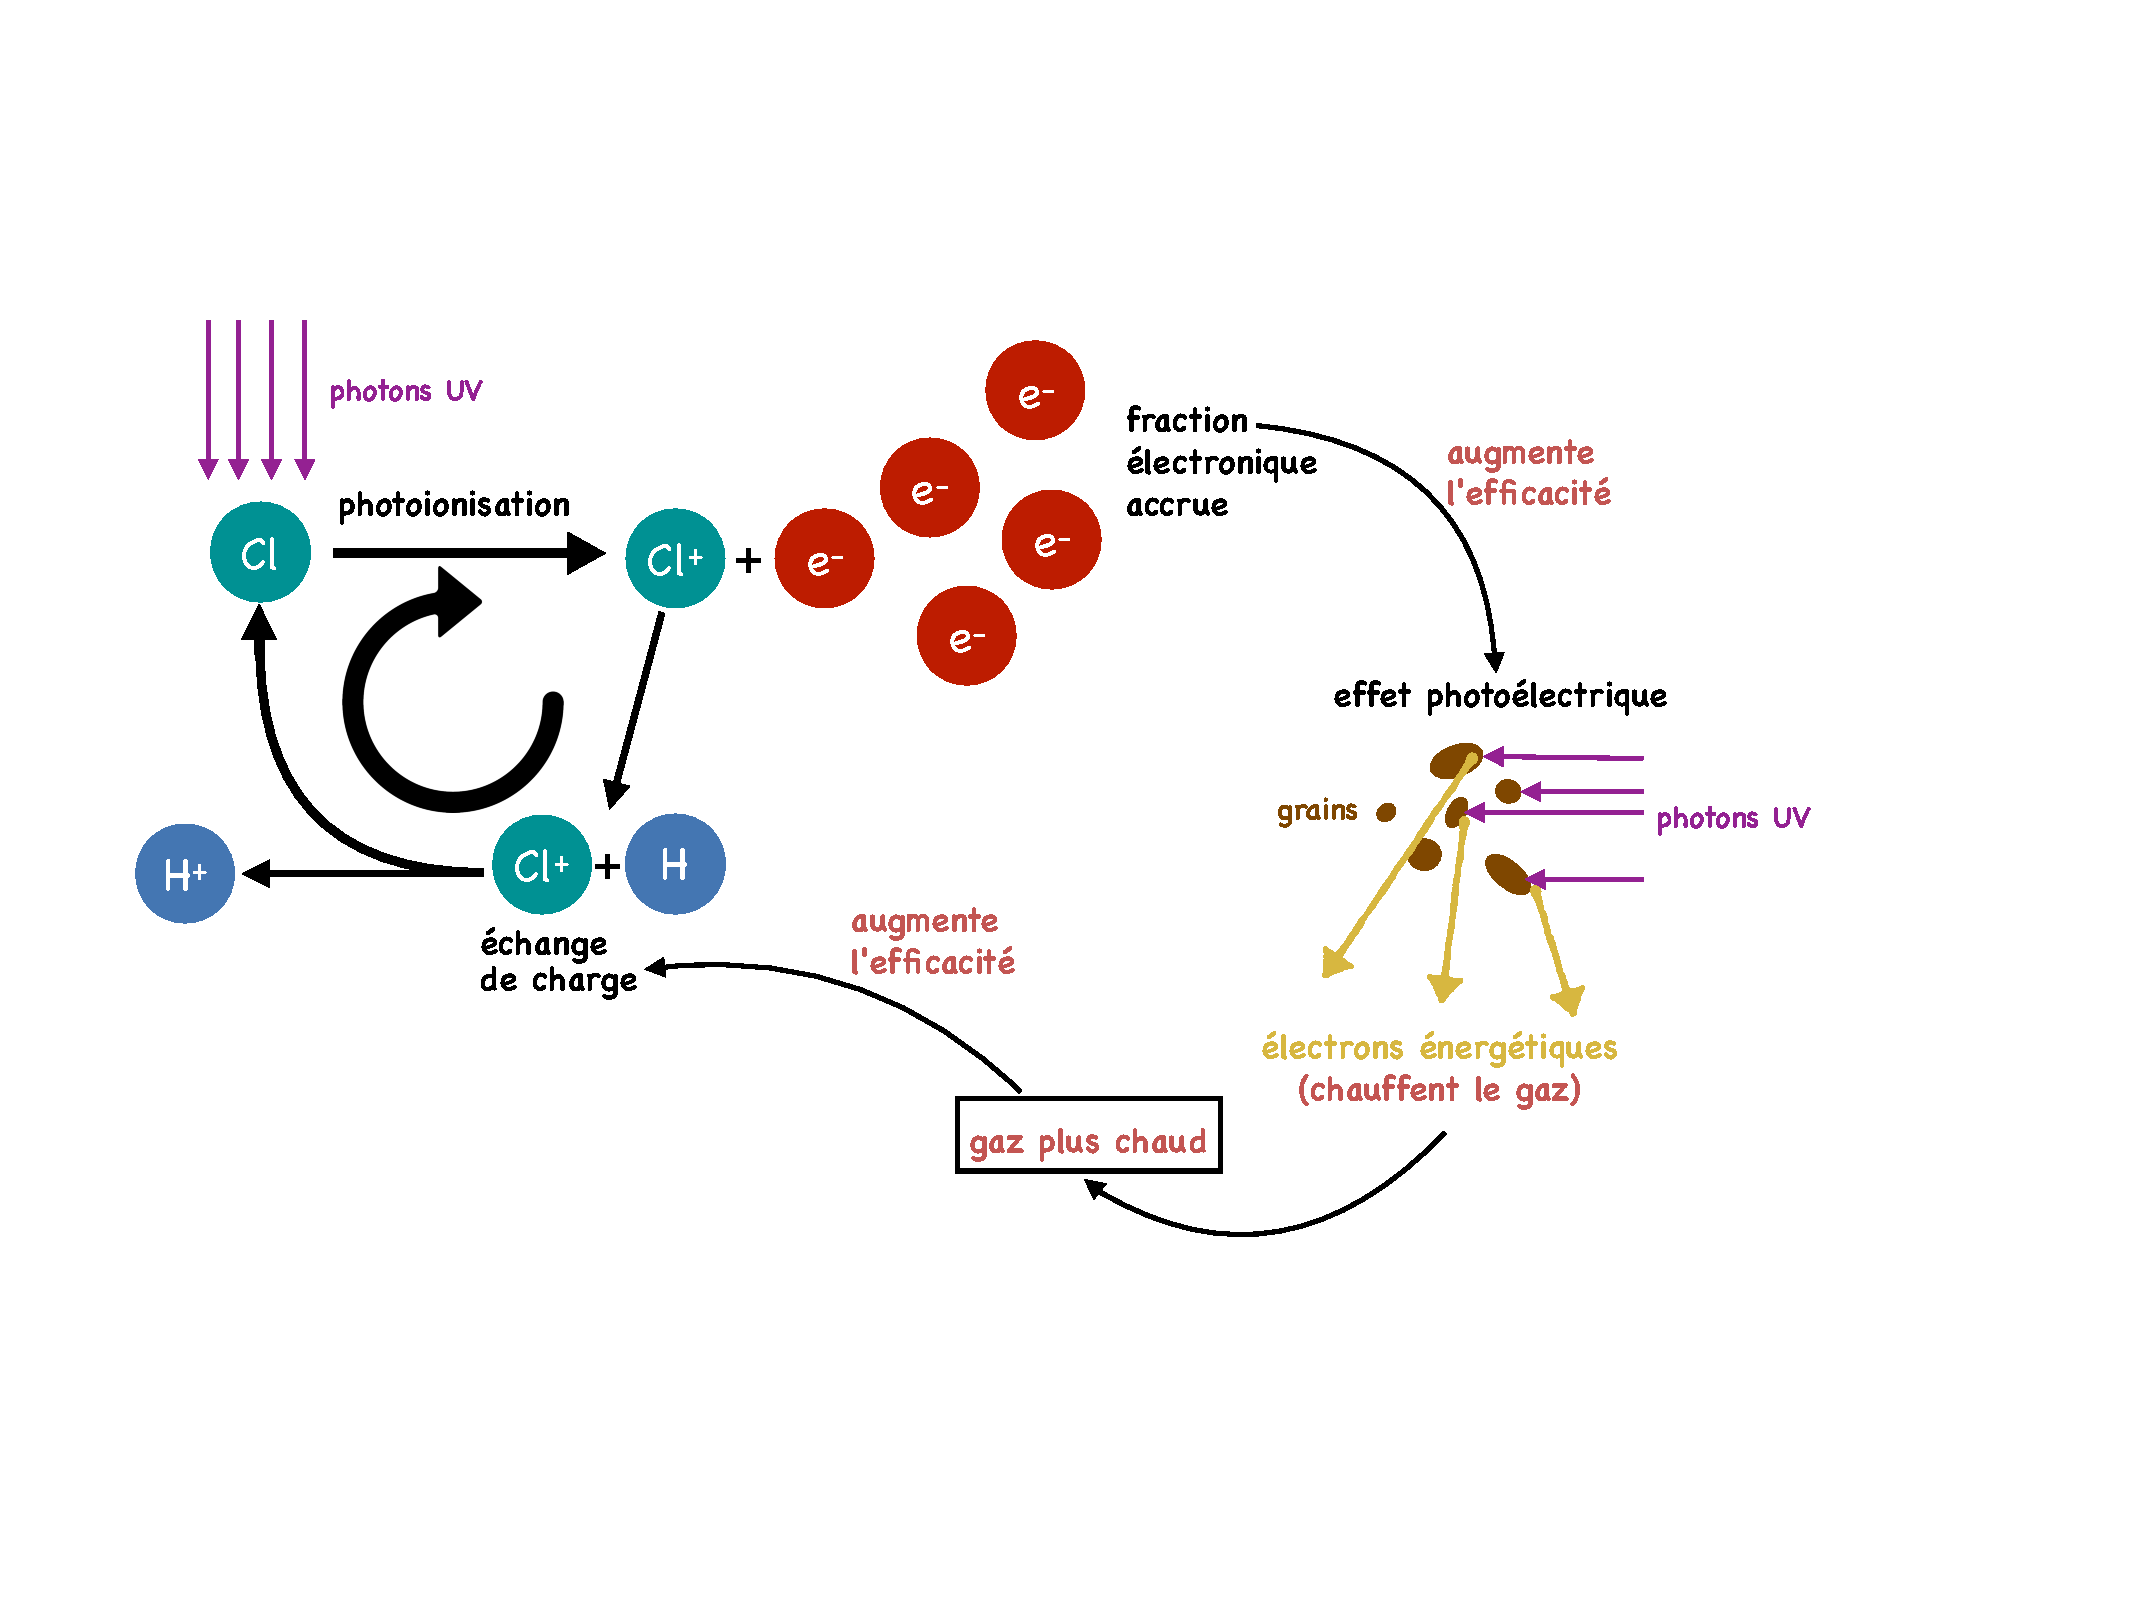
\includegraphics[trim = {2cm 5cm 4cm 4cm},clip, width=0.8\textwidth]{figure/Cl/Cl_heating_fr-5.pdf}
    \caption{Schéma représentant l'impact du chlore sur la chimie de bord de nuage atomique}
    \label{fig:catalyseur}
\end{figure}{}

L'emballement de l'effet photoélectrique se produit à partir de 1000 K. Or la photoionisation du carbone et du soufre produit les électrons en bord de nuage atomique indépendamment de la température. Il existe une température où le transfert de charge devient suffisamment efficace pour que la fraction d'électrons créée via le chlore devienne dominante devant celle de la ionisation du carbone et du soufre et amorce la rétroaction de l'effet photoélectrique. L'amplification dépend donc l'énergie d'activation du transfert de charge $\mathrm{Cl}^+  + \mathrm{H}    \rightarrow \mathrm{Cl}   +  \mathrm{H}^+$ qui vaut 6290 K. \newline

Parmi les espèces figurant dans le modèle, la carbone, le soufre, le silicium ou le fer ont également un potentiel de ionisation inférieur à celui de l'hydrogène (\autoref{tab:gaz}). Pourtant aucun ne peut effectuer un transfert de charge avec l'hydrogène qui est l'espèce majoritaire en bord de nuage atomique. Ces espèces ne peuvent pas donc pas provoquer un emballement similaire à celui induit par le chlore. 


%%%%%%%%%%%%%%%%%%%%%%%%%%%%%%%%%%%%%%%%%%%%%%%%%%%%%%%%%%%%%%%%%%%%%%%%%%%%%%%%%%%%%%%%%%%%%%%


\subsection{Modèle analytique - Chimie}

L'effet photoélectrique sur les grains est le phénomène de chauffage dominant dans les PDR. Son taux, donnée dans \cite{BakesTielens1994}, est $\Gamma_{pe} = 10^{-24}\,\epsilon\,G_0\, n_{\mathrm{H}}$ en $\mathrm{erg}\, \mathrm{s}^{-1} \mathrm{cm}^{-3}$ où $G_0$ est l'intensité du champs UV en Habing ($G_0 = 1.71\chi$) et $\epsilon$ est l'efficacité en $\mathrm{s}^{-1}$ de l'effet photoélectrique : 

\begin{equation}
    \epsilon = \frac{ 3\times 10^{-2}}{1 +  2\times 10^{-4}(G_0\sqrt{T}/n_e)}
\end{equation}

Elle dépend de la température $T$ et de la densité d'électrons $n_e$ dans le nuage. Il faut donc déterminer une expression de la densité d'électrons en fonction de la température. \newline 

Les espèces qui contribuent à la production d'électrons en bord de nuage sont les ions hydrogène $\mathrm{H}^+$, carbone $\mathrm{C}^+$ et soufre $\mathrm{S}^+$. Le gaz est neutre, le bilan de charge donne donc :

\begin{equation}
    n_e = n(\mathrm{H}^+) + n(\mathrm{C}^+) + n(\mathrm{S}^+)
    \label{eq:bilan:ne}
\end{equation}


On peut supposer qu'en entrée de nuage atomique le carbone et le soufre sont totalement ionisés ce qui fournit une fraction d'électrons minimale\footnote{Dans le modèle à $n_{\mathrm{H}} = 10^4\ cm^{-3}$ et $\chi = 10^4$, le code obtient de manière indépendante de la température $n(\mathr{C}^+) = 1.32\,\mathrm{cm}^{-3}$ et $n(\mathr{S}^+) = 1.86\,10^{-1}\,\mathrm{cm}^{-3}$ ce qui donne une fraction électronique $\frac{1}n_\mathrm{H} (n(\mathr{C}^+)+n(\mathr{S}^+) ) = 1.5\,10^{-4} \approx 10^{-4}$ } de $10^{-4}$. Aussi ne reste il qu'à déterminer une expression de la densité de protons $\mathrm{H}^+$ en fonction de la température.
% Le modèle analytique doit retrouver l'augmentation de la densité d'électrons (jusqu'à $2\ 10^{-3}$) pour des températures supérieures à 1000 K. \newline 

\subsubsection{Ion hydrogène}

Les réactions les plus efficaces qui forment et détruisent les ions $\mathrm{H}^+$ en bord atomique de nuage sont :

\begin{equation}\label{eq:sysH}
    \begin{array}{lllllllr}
        \mathrm{Cl}^+ & + &\mathrm{H}   & \rightleftharpoons &\mathrm{Cl}  & + & \mathrm{H}^+ &   \\
        \mathrm{O}^+ & + &\mathrm{H}   & \rightleftharpoons &\mathrm{O}  & + & \mathrm{H}^+ &   \\
        \mathrm{H}^+  & + & \mathrm{e}^-  & \rightarrow &\mathrm{H}   &   &  &  \\
        \mathrm{H}^+  & + & \mathrm{grains}  & \rightarrow &\mathrm{H}   &   &  &  \\
    \end{array}
\end{equation}

Les réactions avec l'oxygène sont négligées car la formation et destruction de $\mathrm{H}^+$ par l'oxygène se compensent totalement en première approximation. De plus le taux de recombinaison de l'ion $\mathrm{H}^+$ sur les grains ($\mathrm{H}^+  + \mathrm{grains}  \rightarrow \mathrm{H}$) est difficile à estimer, on le néglige dans un premier temps. Il reste le transfert de charge entre le chlore et l'hydrogène ($\mathrm{Cl}^+  + \mathrm{H}    \rightleftharpoons &\mathrm{Cl}   +  \mathrm{H}^+$) ainsi que la recombinaison électronique de l'hydrogène ($\mathrm{H}^+  + \mathrm{e}^-  \rightarrow\mathrm{H}$). On associe à chaque réaction un taux de réaction $k_3$,$k_4$, $k_5$ en $\mathrm{cm}^{-3}\,\mathrm{s}^{-1}$ et qui dépendent de la température.  <nommer les coefficients en recommencant de 1 ?>

\begin{equation}
    \begin{array}{lllllllr}
        \mathrm{Cl}^+ & + &\mathrm{H}   & \rightarrow &\mathrm{Cl}  & + & \mathrm{H}^+ & (k_3) \\
        \mathrm{Cl}  & + & \mathrm{H}^+  & \rightarrow & \mathrm{Cl}^+ & + &\mathrm{H}  & (k_4) \\
        \mathrm{H}^+  & + & \mathrm{e}^-  & \rightarrow &\mathrm{H}   &   &     & (k_5) \\
    \end{array}
\end{equation}

A l'état stationnaire, le bilan de formation des ions $\mathrm{H}^+$ donne
\begin{equation}\label{eq:h+}
    \frac{d}{dt}n(\mathrm{H}^+) = k_3n(\mathrm{Cl}^+)n(\mathrm{H}) - k_4n(\mathrm{Cl})n(\mathrm{H}^+) - k_5 n(\mathrm{H}^+)n_e = 0
\end{equation}

En introduisant la fraction atomique de chlore $\delta_{Cl}$, fixée dans le gaz, et le bilan de charge (eq \ref{eq:bilan:ne}) on obtient une équation en $n(\mathrm{H}^+)$ :

\begin{equation}
    -k_3n(\mathrm{Cl}^+)n_{\mathrm{H}} + \bigg( \frac{k_3 k_4}{k_1} n_{\mathrm{H}} n(\mathrm{Cl}^+) + k_5 \big(n(\mathrm{C}^+)+ n(\mathrm{S}^+)\big) \bigg) n(\mathrm{H}^+) + k_5 n(\mathrm{H}^+)^2 = 0
\end{equation}

 avec,
\begin{equation}
    \delta_{Cl} = 1.8\,10^{-7} = \frac{n(\mathrm{Cl}) + n(\mathrm{Cl}^+) + ...}{n(\mathrm{H}) + n(\mathrm{H}^+) + 2n(\mathrm{H}_2) + ...} \approx \frac{1}{n_{\mathrm{H}}} (n(\mathrm{Cl}) + n(\mathrm{Cl}^+) )
\end{equation}

On obtient alors une solution qui dépend de $n(\mathrm{Cl}^+)$,

\begin{equation}
\hspace{-3em}
\resizebox{1.1\hsize}{!}{
    \boxed{n(\mathrm{H}^+) = -\frac{1}{2} \bigg( \frac{k_3 k_4}{k_1 k_5} n_{\mathrm{H}} n(\mathrm{Cl}^+) + n(\mathrm{C}^+)+ n(\mathrm{S}^+) \bigg) \pm \frac{1}{2} \sqrt{\bigg( \frac{k_3 k_4}{k_1 k_5} n_{\mathrm{H}} n(\mathrm{Cl}^+) + n(\mathrm{C}^+)+ n(\mathrm{S}^+) \bigg)^2 + 4\frac{k_3}{k_5}n_{\mathrm{H}} n(\mathrm{Cl}^+)}}
    }
\end{equation}

% \subsubsection{Rôle de l'oxygène}
% Au vu des taux de réactions impliquant le $\mathrm{H}^+$ nous pourrions choisir d'inclure la chimie de $\mathrm{H}^+$ avec l'oxygène. A hautes températures, les taux de $ \mathrm{H}^+ + O \leftrightarrows\mathrm{H}+ O^+ \quad (k_6,k_7)$ prédominent sur les autres réactions. Si l'on considère que ces réactions pour la chimie de l'oxygène, les $\mathrm{H}^+$ produits seront consommés pour former du $H$. Rien ne se passe. Pour s'en convaincre il suffit d'écrire la nouvelle équation bilan de $\mathrm{H}^+$ et d'utiliser celle pour $O^+$.

% \begin{equation}
%     \frac{d}{dt}n(O^+) = k_6 n(\mathrm{H}^+)n(O) - k_7n(\mathrm{H})n(O^+) = 0
% \end{equation}

% En l'injectant dans le nouveau bilan de formation pour le $\mathrm{H}^+$, ces nouveaux termes disparaissent. Cependant si l'on calcule l'expression de $n(\mathrm{H}^+)$ à partir des concentrations de $n(O^+)$ et $n(O)$, l'approximation donne une meilleure correspondance avec l'abondance calculé par le code. 

% \begin{equation}
%     n(\mathrm{H}^+) =  \frac{k_3 n_{\mathrm{H}} n(\mathrm{Cl}^+) + k_6 n_{\mathrm{H}} n(O^+) }{k_5 n(\mathrm{e}^-) + k_4 \frac{n(\mathrm{Cl}^+)}{A} + k_7 n(O) }
% \end{equation}

% Utiliser les abondances de l'oxygène demande d'étudier sa chimie, et donc de prendre en compte d'autres espèces comme $OH$ ou $O_2$ ce qui complexifie le modèle. 

%%%%%%%%%%%%%%%%%%%%%%%%%%%%%%%%%%%%%%%%%%%%%%%%%%%%%%%%%%%%%%%%%%%%%%%%%%%%%%%%%%%%%%%%%%%%%%

\subsubsection{Ion chlore}

De la même manière, les réactions importantes faisant intervenir le chlore sont :

\begin{equation}\label{eq:sysCl}
    \begin{array}{lllllllr}
        \mathrm{Cl}^+ & + &\mathrm{H}   & \rightleftharpoons &\mathrm{Cl}  & + & \mathrm{H}^+ &   \\
        \mathrm{Cl}^+ & + &\mathrm{H_2}   & \rightarrow & \mathrm{HCl}^+ & + &  \mathrm{H}&  \\
       \mathrm{Cl}  & + & h\nu & \rightleftharpoons & \mathrm{Cl}^+ & + & \mathrm{e}^- &  \\
    \end{array}
\end{equation}


La recombinaison électronique de $\mathrm{Cl}^+$ ($\mathrm{Cl}^+ + \mathrm{e}^-\rightarrow & \mathrm{Cl} + h\nu $) reste négligeable devant le transfert de charge avec $\mathrm{H}$  ($\mathrm{Cl}^+ + \mathrm{H} \rightarrow & \mathrm{Cl}+ \mathrm{H}^+ $) pour des températures supérieure à $100$K et la destruction par formation du $\mathrm{HCl}^+$ devient dominante dans la gamme de température $100-1000$K. Négliger ces réactions donne une approximation correcte de la densité d'ion chlore pour les régimes de températures $T\geq 1000$ K et garde l'emballement de l'effet photoélectrique. On considère ainsi les réactions ci-dessous avec les taux de réactions $k_1$ en $\mathrm{s}^{-1}$ et $k_3$ en $\mathrm{cm}^{-3}\,\mathrm{s}^{-1}$.

\begin{equation}
    \begin{array}{lccccclr}
       \mathrm{Cl}  & + & h\nu & \rightarrow & \mathrm{Cl}^+ & + & \mathrm{e}^- & (k_1) \\
        \mathrm{Cl}^+ & + &\mathrm{H}   & \rightarrow &\mathrm{Cl}  & + & \mathrm{H}^+ & (k_3) \\
    \end{array}
\end{equation}

Un travail similaire nous donne 
\begin{equation}
    k_1(\delta_{Cl}n_{\mathrm{H}} - n(\mathrm{Cl}^+)) - k_3 n(\mathrm{Cl}^+) n_{\mathrm{H}} = 0
\end{equation}

Ce qui fait en posant $A = \frac{k_1}{k_3 n_{\mathrm{H}}}$:

\begin{equation}
\boxed{n(\mathrm{Cl}^+) = \frac{k_1 \delta_{Cl} n_{\mathrm{H}}}{k_1 + k_3 n_{\mathrm{H}}} = \frac{A}{1 + A} \delta_{cl} n_{\mathrm{H}}}
\end{equation}


%%%%%%%%%%%%%%%%%%%%%%%%%%%%%%%%%%%%%%%%%%%%%%%%%%%%%%%%%%%%%%%%%%%%%%%%%%%%%%%%%%%%%%%%%%%%%%%

\subsubsection{Recombinaison de $\mathrm{H}^+$ sur les grains}

Le taux de recombinaison du $\mathrm{H}^+$ sur les grains est calculé dans le code à partir de la distribution des grains : nous n'avons pas d'expression explicite pour notre modèle. Par ailleurs, sans la recombinaison, le modèle semi-analytique surestime la densité d'électrons aux hautes températures. On utilise donc une expression calculé à partir de données observationelles et qui considère une population de grains différente de celle du code (équations [5][8] de \cite{Weingartner_2001}). 

\begin{equation}
    \alpha \left(\mathrm{X}^{i}, \psi, T\right) \approx \frac{10^{-14} C_{0} }{1+C_{1} \psi^{C_{2}}\left(1+C_{3} T^{C_{4}} \psi^{-C_{5}-C_{6} \ln T}\right)} \quad \mathrm{cm}^{3} \mathrm{s}^{-1}
\end{equation}

avec $\psi = \frac{G_0 \sqrt{T}}{n_e}$. Les coefficients $\mathrm{C}_i$ sont des paramètres de fit. Le bilan eq.\ref{eq:h+} devient : 

\begin{equation}\label{eq:h+}
    \frac{d}{dt}n(\mathrm{H}^+) = k_3n(\mathrm{Cl}^+)n(\mathrm{H}) - k_4n(\mathrm{Cl})n(\mathrm{H}^+) - k_5 n(\mathrm{H}^+)n_e -\alpha n(\mathrm{H}^+)n_{\mathrm{H}} = 0
\end{equation}

où $\alpha$ est fonction de $n_e$. On obtient une équation implicite en fonction de la densité d'électrons qui vérifie :
\begin{equation}
    x = n(\mathrm{H}^+)(x) + n(\mathrm{S}^+)  + n(\mathrm{C}^+)
\end{equation}

La fonction \texttt{newton} de la librairie \texttt{scipy.optimize} vient à bout de ce système. On visualise sur la figure \ref{fig:Cl:model:rec} les densités d'électrons calculés par le modèle semi-analytique et par le code PDR. La formule de \cite{Weingartner_2001} considère dans le nuage une distribution de grains incluant les PAH\footnote{Les PAH sont des \textit{Polycyclic Aromatic Hydrocarbons} qui sont des structures planes de carbones organisés en anneaux hexagonaux avec des atomes d'hydrogène liés aux extrémités. Ils ont une taille inférieure à environ $5\,\mathrm{nm}$ \cite{DraineBook}.} qui est un support efficace pour la recombinaison des ions $\mathrm{H}^+$. On voit en effet sur la figure \ref{fig:Cl:model:recPAH} qu'avec les
PAH le modèle semi-analytique surestime la densité d'électrons prédite par le code PDR tandis qu'en prenant en compte l'expression de \cite{Weingartner_2001} on obtient une densité proche de celle du code. Si l'on ne prend pas en compte les PAH dans le code PDR (figure \ref{fig:Cl:model:recnoPAH}), le code PDR utilise moins de petits grains que la formule et il est nécessaire de diminuer le taux de recombinaison d'un facteur $1/6$ pour approcher la densité d'électrons calculé par le code.


% La densité d'électrons calculée montré sur la figure \ref{fig:Cl:model:rec}. On a résolu le système dans deux cas. Un cas avec les PAH (fraction massique = $4.6\,10^{-2}$) où le taux de recombinaison donné \cite{Weingartner_2001} donne une bonne estimation de la densité d'électrons. Un second cas sans PAH, où il faut réduire d'un facteur $1/6$ la recombinaison de $\mathrm{H}^+$ sur les grains. On avait toujours $r_{\mathrm{min}} = 1\,10^{-7}\,\mathrm{m}$ et $r_{\mathrm{max}} = 3\,10^{-5}\,\mathrm{m}$.

% \textit{Quel réaction réduit la densité d'électrons à très hautes températures et qui nous empêche d'avoir la tangente horizontale ?}
% \textit{C'est du à quoi la production au milieu déjà}

\begin{figure}[!h]
    \centering
    \begin{subfigure}[t]{0.49\textwidth} % "0.49" donne ici la largeur de l'image
        \centering 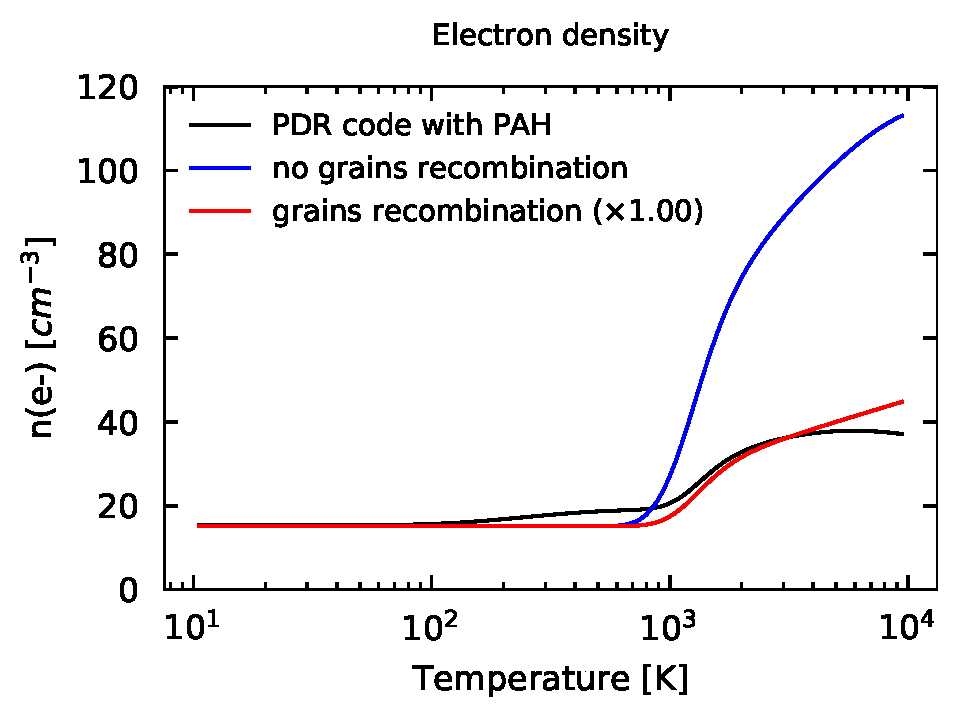
\includegraphics[trim = {0 0 0 1cm},clip,width=1\textwidth]{figure/Cl/test_calc_PAH_e.pdf}
        \caption{avec PAH}
        \label{fig:Cl:model:recPAH}
    \end{subfigure}
    ~ 
    \begin{subfigure}[t]{0.49\textwidth}
        \centering 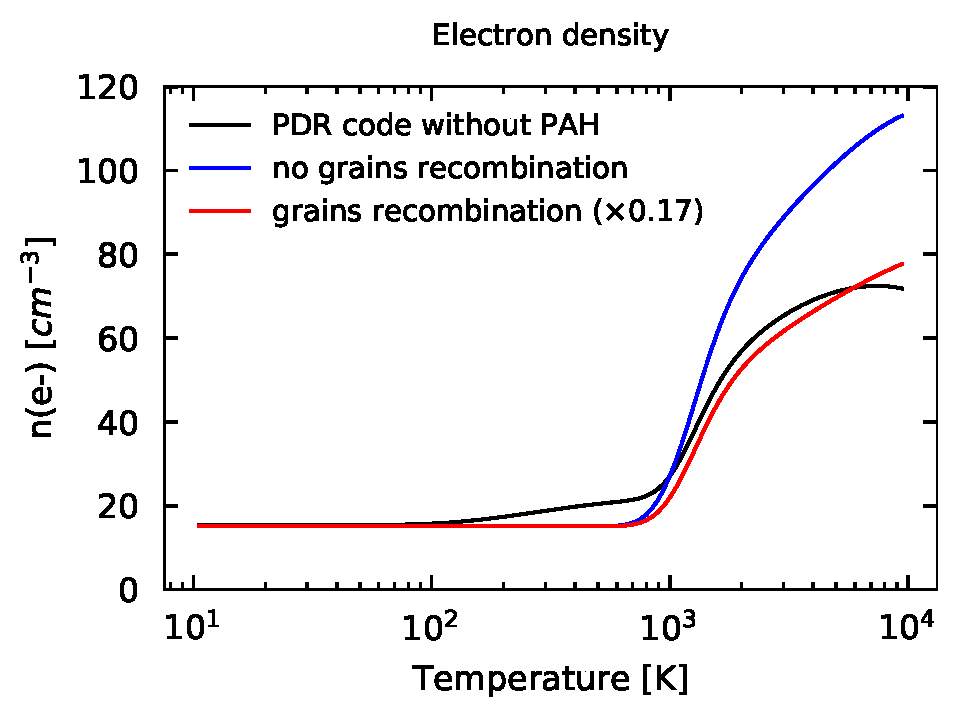
\includegraphics[trim = {0 0 0 1cm},clip,width=1\textwidth]{figure/Cl/test_calc_e.pdf}
        \caption{sans PAH}
        \label{fig:Cl:model:recnoPAH}
    \end{subfigure}
    \caption{Comparaison des profils de densité d'électrons en fonction de la température}
    % \begin{minipage}{\textwidth}
    % \end{minipage}
    \label{fig:Cl:model:rec}
\end{figure}



%%%%%%%%%%%%%%%%%%%%%%%%%%%%%%%%%%%%%%%%%%%%%%%%%%%%%%%%%%%%%%%%%%%%%%%%%%%%%%%%%%%%%%%%%%%%%%%%%%%%%%%%%%%%%%%%%%%%%%%%%%%%%%%%%%%%%%%%%%%%%%%%%%%%%%%%%%%%%%%%%%%%%%%%%%%%%%%%%%%%%%%%%%

\subsection{Modèle analytique - Thermique}

Pour construire un bilan thermique et déterminer la température d'équilibre du gaz, il faut considérer les processus de chauffage et refroidissement qui interviennent en bord atomique des nuages. Les processus thermiques employés dans le modèle sont :

\begin{itemize}
    \item le chauffage net de l'effet photoélectrique sur les grains (\cite{BakesTielens1994})
    % \item la recombinaison électronique sur les grains
    \item le refroidissement par émission de raies de structure fine du [CII] $158 \mu m$,  [OI]$63 \mu m$, [OI]$6300A$ (\cite{Rollig2005})
    \item l'émissions Lyman $\mathrm{H}\alpha$ (\cite{tielens2005})
    \item le couplage gaz-grain (\cite{Hollenbach1991}).
\end{itemize}{}

Les processus thermiques impliquant la molécule $\mathrm{H}_2$ ont été négligé car ils demandent de connaître la densité de $\mathrm{H}_2$ dans le bord atomique du nuage. On dénote $\Gamma$ et $\Lambda$ les taux de chauffage et de refroidissement total.

\begin{equation}
    \begin{split}
        \Gamma &= \Gamma_{pe}^{\mathrm{net}} \\
        \Lambda &=   \Lambda_{\mathrm{CII}\ 158 \mu \mathrm{m}} + \Lambda_{\mathrm{OI}\ 63 \mu \mathrm{m}} + \Lambda_{\mathrm{OI}\ 146 \mu \mathrm{m}}  + \Lambda_{\mathrm{H}_\alpha} + \Lambda_{\mathrm{g}-\mathrm{g}} 
    \end{split}
\end{equation}

%%%%%%%%%%%%%%%%%%%%%%%%%%%%%%%%%%%%%%%%%%%%%%%%%%%%%%%%%%%%%%%%%%%%%%%%%%%%%%%%%%%

\subsubsection{Chauffage net par effet photoélectrique sur les grains}

Quand un photon qui a suffisamment d'énergie est absorbé par un grain, un électron peut être excité et être éjecté de la surface du grain. Ce photoélectron a une énergie de l'ordre de l'eV ($1\,\mathrm{eV}\approx 50\,000$K) et vient chauffer le gaz par thermalisation à un taux $\Gamma_{\mathrm{pe}}$. Il y a également le phénomène inverse : la recombinaison des électrons et des ions (principalement $\mathrm{H}^+$ et $\mathrm{C}^+$) sur les grains fait perdre de l'énergie au gaz à un taux $\Lambda_{\mathrm{rec}}$ \cite{Lequeux}. Ces phénomènes dépendent principalement de l'intensité du champs de rayonnement $\chi$ et de la charge de grain, c'est à dire le bilan de charge des grains dans le nuage, car il est par exemple plus difficile de prélever des photoélectrons et plus efficace de recombiner sur des grains positivement chargés. Le taux de chauffage net des grains s'écrit $\Gamma^{\mathrm{net}}_{\mathrm{pe}} = \Gamma_{\mathrm{pe}} - \Lambda_{\mathrm{rec}}$. On se contente d'utiliser les formules de \cite{BakesTielens1994} :

\begin{equation}
    \Gamma_{\mathrm{pe}} = 10^{-24}\,G_0\,n_\mathrm{H}\, \frac{2\times 10^{-2}}{1 + 2\times 10^{-4}\,(G_0 \sqrt{T}/n_e)} \qquad \operatorname{erg} \mathrm{cm}^{-3} \mathrm{s}^{-1}
    \label{eq:Rollig:pe}
\end{equation}

\begin{equation}
    \Lambda_{\mathrm{rec}} = 3.49\,10^{-30} T^{0.944} \, (\frac{G_0 \sqrt{T}}{n_e})^{0.735 T^{-0.068}} \, n_e \, n_\mathrm{H} \qquad \operatorname{erg} \mathrm{cm}^{-3} \mathrm{s}^{-1}
    \label{eq:Rollig:rece}
\end{equation}

avec $G_0 = 1.71\chi$.
% (\cite{Wolfire_2003} Eq 20, \cite{BakesTielens1994}) propose une autre formule prenant en compte les PAH qui est de la forme 
% \begin{equation}
%     \Gamma_{\mathrm{pe}}^{\mathrm{Wolf}} = 10^{-24}\,G_0\,n_\mathrm{H}\, \bbig[ \frac{4.9\times 10^{-2}}{1 + 4\times 10^{-3}\, \frac{G_0 \sqrt{T}}{n_e \phi_\mathrm{PAH}}} + \frac{3.7\times 10^{-2} (T/10^4)^{0.7}}{1 + 2\times 10^{-4}\, \frac{G_0 \sqrt{T}}{n_e \phi_\mathrm{PAH}}} \bbig]\qquad  \operatorname{erg} \mathrm{cm}^{-3} \mathrm{s}^{-1}
% \end{equation}
% avec $\phi_\mathrm{PAH}$ une efficacité de collision compris entre 0 et 1. L'effet photoélectrique est d'autant plus efficace sur les petits grains \cite{DraineBook}. Le choix de $r_\mathrm{min}$ (la taille minimale des grains dans la description MRN) est décisif. Si l'on trace ces formules sur la \autoref{fig:Cl:pePAH} pour différent $\phi_\mathrm{PAH}$ et $r_\mathrm{min}$ on voit que la formule de \cite{Rollig2005} sous-estime le taux calculé par le code PDR de Meudon. Avec $r_\mathrm{min} = 1\,10^7\,\mathrm{nm}$, la prescription de Rollig est 3 fois plus petit que le chauffage calculé par Meudon. Si l'on augmente la taille de grain minimale, on voit que cette écart diminue ce qui est cohérent car on enlève des petits grains. La prescription de \cite{Wolfire_2003} laisse plus de liberté à travers le $\phi_\mathrm{PAH}$ (à mieux dire).
% \begin{figure}[!h]
%     \centering
%     \begin{subfigure}[t]{0.49\textwidth} % "0.49" donne ici la largeur de l'image
%         \centering 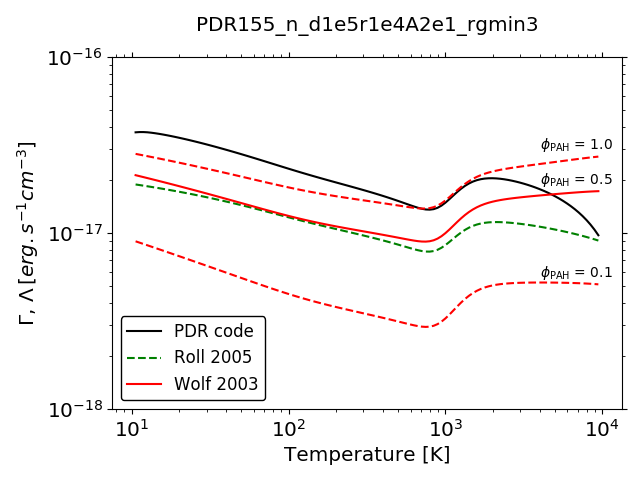
\includegraphics[trim = {0 0 0 1cm},clip,width=1\textwidth]{figure/Cl/pePAH/pe_formulae_rgmin3.png}
%         \caption{$r_\mathrm{min} = 3\,10^{-7} \, \mathrm{nm}$}
%     \end{subfigure}
%     ~ 
%   \begin{subfigure}[t]{0.49\textwidth} % "0.49" donne ici la largeur de l'image
%         \centering 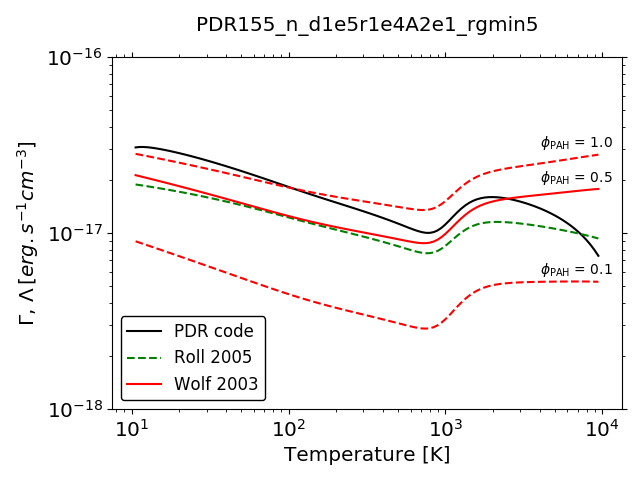
\includegraphics[trim = {0 0 0 1cm},clip,width=1\textwidth]{figure/Cl/pePAH/pe_formulae_rgmin5.png}
%         \caption{$r_\mathrm{min} = 5\,10^{-7}\, \mathrm{nm}$}
%     \end{subfigure}
%     \caption{Comparaison des formules de l'effet photoélectrique de \cite{Rollig2005} et \cite{Wolfire_2003} avec le code PDR pour différents $r_\mathrm{min}$}
%     \label{fig:Cl:pePAH}
% \end{figure}
%
% Il existe également celle ci \cite{WolfireHollenbachMcKeeTielensBakes_1995} Eq. 9 que l'on n'utilise pas.

% \begin{equation}
%     \Lambda_{\mathrm{rec}}^{\mathrm{Wolfire}} = 4.65\,10^{-30} T^{0.94} \, (\frac{G_0 \sqrt{T}}{n_e})^{\frac{0.74}{T^{0.068}}} \, n_e \, n_\mathrm{H} \qquad \operatorname{erg} \mathrm{cm}^{-3} \mathrm{s}^{-1}
% \end{equation}


% \cite{Rollig2005} (Eq (10) ou (C.3)) qui provient de \cite{BakesTielens1994}, sans PAH, on utilise : 

% \begin{equation}
%     \Gamma_{\mathrm{pe}} = 10^{-24}\,G_0\,n_\mathrm{H}\, \frac{2\times 10^{-2}}{1 + 2\times 10^{-4}\,G_0 \sqrt{T}/n_e} \qquad \operatorname{erg} \mathrm{cm}^{-3} \mathrm{s}^{-1}
%     \label{eq:Rollig:pe}
% \end{equation}

% Avec $G_0 = 1.71\chi \times 0.5$ car il considère une illumination provenant que d'un coté. 

% Dans le modèle de chlore, on prend celle de \cite{Rollig2005} Eq.4  qui provient elle même de \cite{BakesTielens1994}.

% \begin{equation}
%     \Lambda_{\mathrm{rec}} = 3.49\,10^{-30} T^{0.944} \, (\frac{G_0 \sqrt{T}}{n_e})^{\frac{0.735}{T^{0.068}}} \, n_e \, n_\mathrm{H} \qquad \operatorname{erg} \mathrm{cm}^{-3} \mathrm{s}^{-1}
%     \label{eq:Rollig:rece}
% \end{equation}
%%%%%%%%%%%%%%%%%%%%%%%%%%%%%%%%%%%%%%%%%%%%%%%%%%%%%%%%%%%%%%%%%%%%%%%%%%%%%%%%%%%%%%%%%%%%%%%

\subsubsection{Refroidissement par les raies d'émissions du $\mathrm{C}^+$ et de $\mathrm{O}$}

Les collisions entre les particules du gaz peuvent peupler les niveaux excités des espèces. S'il s'en suit une désexcitation par une collision le bilan d'énergie prélevé au gaz est nul. Tandis que s'il s'en suit une émission spontanée d'un photon, de l'énergie a été perdu par le gaz. On utilise les expression de \cite{Rollig2005} qui estime le refroidissement des raies [CII]$158 \mu \mathrm{m}$, [OI]$62 \mu \mathrm{m}$ et [OI]$146 \mu \mathrm{m}$.

\begin{equation}
    \Lambda_{\mathrm{CII}\ 158   \mu \mathrm{m}}= n(\mathrm{C}^+) \frac{2.89 \times 10^{-20}}{1+\frac{1}{2} \exp (92 / T)\left(1+\frac{1300}{n_\mathrm{H}}\right)} \qquad \operatorname{erg} \mathrm{cm}^{-3} \mathrm{s}^{-1}
\end{equation}

\begin{equation}
\begin{split}
    \Lambda_{\mathrm{OI}\ 63 \mu \mathrm{m}} &= 3.15\,10^{-14} \times 8.46\,10^{-5} \times 
    n(\mathrm{O}) \\
    & \times \frac{e^{98/T} 3 n_\mathrm{H} (n_\mathrm{H} + \beta\, n_{\mathrm{cr}_{01}} ) }{{n_\mathrm{H}}^2+ e^{98/T}(n_\mathrm{H} + \frac{1}{2} n_{\mathrm{cr}_{01}} ) (3 n_\mathrm{H} + 5\, e^{228/T} (n_\mathrm{H} + \frac{1}{2} n_{\mathrm{cr}_{12}} )) } \qquad \operatorname{erg} \mathrm{cm}^{-3} \mathrm{s}^{-1}
\end{split}
\end{equation}

\begin{equation}
\begin{split}
    \Lambda_{\mathrm{OI}\ 146 \mu \mathrm{m}} &= 1.35\,10^{-14} \times 8.46\,10^{-5} \times 
    n(\mathrm{O}) \\
    & \times \frac{ {n_\mathrm{H}}^2 }{n_\mathrm{H}^2+ e^{98/T}(n_\mathrm{H} + \frac{1}{2} n_{\mathrm{cr}_{01}} ) (3 n_\mathrm{H} + 5\, e^{228/T} (n_\mathrm{H} + \frac{1}{2} n_{\mathrm{cr}_{12}} )) } \qquad \operatorname{erg} \mathrm{cm}^{-3} \mathrm{s}^{-1}
\end{split}
\end{equation}

Avec $n_{\mathrm{cr}_{01}}(T) = \frac{1.66\,10^{-5} }{1.35\,10^{-11} T^{0.49}} $ et $n_{\mathrm{cr}_{12}}(T) = \frac{8.46\,10^{-5} }{4.37\,10^{-12} T^{0.66}} $

%%%%%%%%%%%%%%%%%%%%%%%%%%%%%%%%%%%%%%%%%%%%%%%%%%%%%%%%%%%%%%%%%%%%%%%%%%%%%%%%%%%%%%%%%%%%%%%
\subsubsection{Couplage gaz-grains}

De \cite{Rollig2005} ($Z=1$), le couplage gaz grain s'exprime,

\begin{equation}
    \Lambda_{\mathrm{g}-\mathrm{g}} = 3.5\,10^{-34}\times \sqrt{T}(T - T_g) {n_\mathrm{H}}^2 \qquad \operatorname{erg} \mathrm{cm}^{-3} \mathrm{s}^{-1}
\end{equation}

Où $T_g$ est donné par Eq. 6 de \cite{HollenbachTakahashiTielens_1991}
\begin{equation}
    T_g = 12.2 \,{G_0}^{0.2}
\end{equation}


%%%%%%%%%%%%%%%%%%%%%%%%%%%%%%%%%%%%%%%%%%%%%%%%%%%%%%%%%%%%%%%%%%%%%%%%%%%%%%%%%%%%%%%%%%%%%%%

\subsubsection{Emission Lyman $\mathrm{H}\alpha$}

\cite{tielens2005}, Eq 2.62

\begin{equation}
    \Lambda_{\mathrm{H}\alpha} = 7.3\, 10^{-19}\,n_e\,n_\mathrm{H}\,e^{-118400/T} \qquad \operatorname{erg} \mathrm{cm}^{-3} \mathrm{s}^{-1}
\end{equation}

%%%%%%%%%%%%%%%%%%%%%%%%%%%%%%%%%%%%%%%%%%%%%%%%%%%%%%%%%%%%%%%%%%%%%%%%%%%%%%%%%%%%%%%%%%%%%%%


%%%%%%%%%%%%%%%%%%%%%%%%%%%%%%%%%%%%%%%%%%%%%%%%%%%%%%%%%%%%%%%%%%%%%%%%%%%%%%%%%%%%%%%%%%%%%%%

\subsection{Correction de l'effet photoélectrique par le code}

Grâce aux expressions de chauffage et de refroidissement ainsi qu'au modèle semi-analytique, le modèle est capable de calculer la température d'équilibre du gaz. Elle est définie telle que $\Gamma(T_{\mathrm{eq}}) - \Lambda(T_{\mathrm{eq}}) = 0$ et est stable (instable) si autour de $T_{\mathrm{eq}}$, $\frac{d}{dT}(\Gamma - \Lambda)$ est négatif (positif). \newline 

On trace sur la figure \ref{fig:Cl:modelPE:GC} la courbe de chauffage et de refroidissement d'un bord atomique de nuage résolu par le code PDR. On trace également les courbes obtenues par notre modèle et on remarque qu'elles retrouvent l'emballement de l'effet photo-électrique à partir de $1000$ K. Néanmoins, on constate que le calcul de Rollig (eq \ref{eq:Rollig:pe}) sous-estime d'un facteur 3 l'effet photo-électrique calculé par le code si bien que le modèle prédit une solution \og chaude \fg{} $4000$ K plus froide que celle obtenue par le code. \newline 
% Par ailleurs la température maximale calculé par notre modèle étant proche de la température du nuage ne comportant pas de chlore, le modèle ne peut pas prédire qu 

Il est prévisible que la formule de Rollig (eq.\ref{eq:Rollig:pe}) diffère de l'effet photoélectrique calculé par le code PDR. En effet, ce processus dépend des paramètres de grains choisis et le code PDR traite les grains de façon plus détaillé que l'expression analytique de Rollig. Cette formule retrouve pourtant l'emballement à hautes températures et a la même allure que le taux calculé par le code PDR. On constate sur la figure \label{fig:Cl:modelPE:GC3} que l'expression eq.\ref{eq:Rollig:pe}, multipliée par un facteur 3, retrouve celle du code et obtient une solution "chaude" proche ($+1500$ K) de celle du code. On gardera désormais cette correction. 


\begin{figure}[!h]
    \centering
    \begin{subfigure}[t]{0.49\textwidth} % "0.49" donne ici la largeur de l'image
        \centering 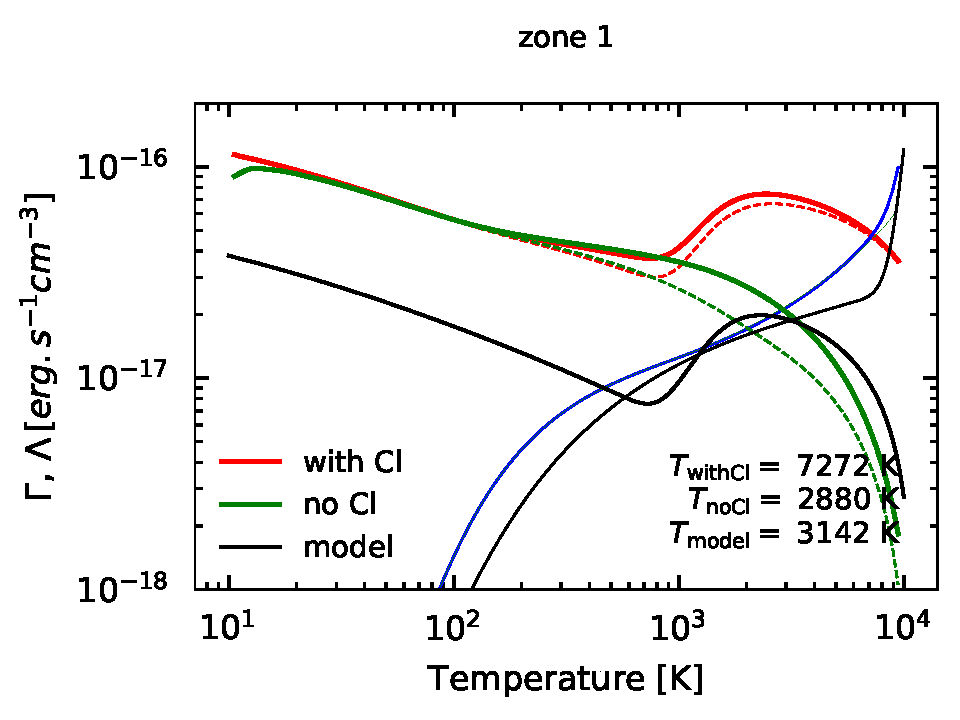
\includegraphics[trim = {0 0 0 1cm },clip,width=1\textwidth]{figure/Cl/modelPE/GCcomp_Cl_1_1.pdf}
        \caption{$\Gamma =  \Gamma_{pe}$}
    \label{fig:Cl:modelPE:GC}
    \end{subfigure}
    ~ 
    \begin{subfigure}[t]{0.49\textwidth}
        \centering 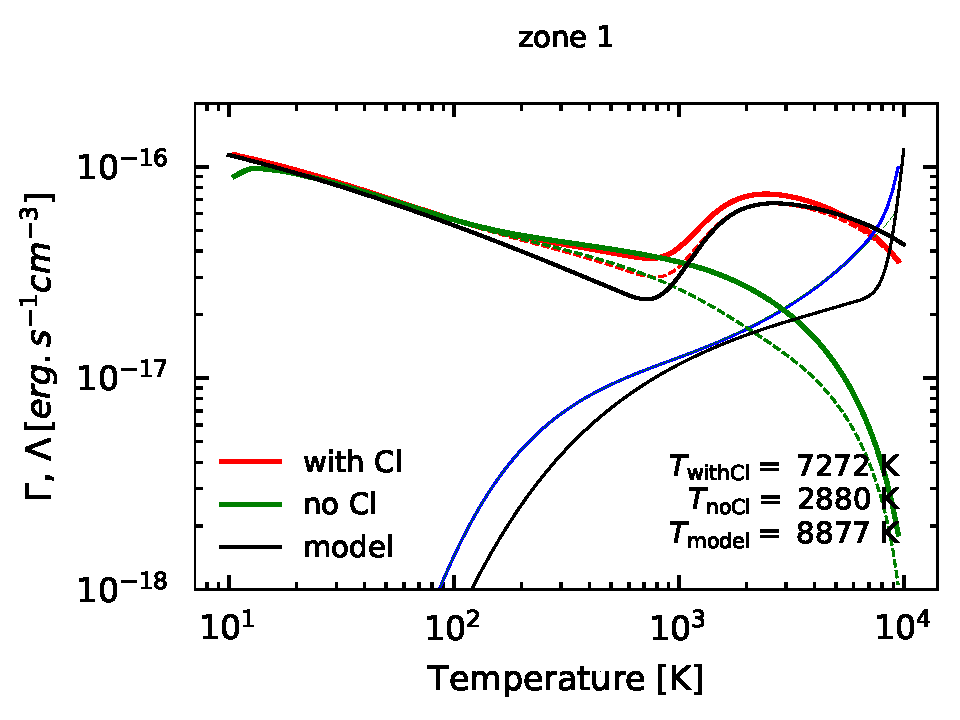
\includegraphics[trim = {0 0 0 1cm },clip,width=1\textwidth]{figure/Cl/modelPE/GCcomp_Cl_1_3.pdf}
        \caption{$\Gamma =  3 \times \Gamma_{pe}$}
    \label{fig:Cl:modelPE:GC3}
    \end{subfigure}
    \caption{Courbes de chauffage et refroidissement au bord atomique d'un modèle à densité constante ($n_\mathrm{H} = 10^{4.5} \,\mathrm{cm}^{-3}$ et $\chi = 10^4$). Le trait en pointillé rouge et vert représente l'effet photoélectrique pour le modèle comportant ou non du chlore.  Le trait plein est le chauffage total. L'écart entre le trait plein et pointillé est dû au chauffage par $\mathrm{H}_2$ qui est mineur ici. Les courbes de refroidissements sont en bleues et quasi-identiques selon qu'il y ait du chlore ou non. La courbe en trait noir est le terme de chauffage du modèle, c'est à dire l'effet photoélectrique sur les grains, calculé par la formule de Rollig. La courbe de refroidissement du modèle est en trait fin noir.}
    
\end{figure}

\subsection{Prédiction de la température au bord de nuage}
 
A l'aide du modèle de chlore nous pouvons chercher dans quelles conditions ($n_\mathrm{H}$ et $\chi$) les bords atomiques des PDR subissent l'instabilité induite par le chlore. Pour étudier globalement les PDR, on utilise des grilles de modèles qui varient dans l'espace des paramètres (densité $n_\mathrm{H}$ et le champ de rayonnement de l'étoile proche $\chi$). Le code PDR résout chaque modèle puis l'on représente une donnée - la température au bord de nuage ou le processus thermique dominant au bord du nuage - dans l'espace des paramètres. On préfère étudier des modèles à densités constantes qui sont plus facile à interpréter (la pression et la température suivent les mêmes variations $\mathrm{P}\propto \mathrm{T}$) que les modèles isobares (la densité et la température varient de manière inversement proportionelle $\mathrm{n}_\mathrm{H}\mathrm{T}=\mathrm{cte}$). 


\subsubsection{Carte de température au bord du nuage}

La figure \ref{fig:Cl:gridModel:Tba} représente la température d'équilibre maximale calculée par le modèle semi-analytique. On constate que les bords atomiques des régions fortement illuminées chauffent en présence du chlore de plusieurs milliers de Kelvin. 
Il apparaît également des instabilités thermiques dans les régions diffuses et fortement illuminées ($n_\mathrm{H} \leq 10^4 \, \mathrm{cm}^{-3}$ et $\chi \geq 10^2$) . Les cartes de température de la figure \ref{fig:Cl:grid:Tba} sont calculées grâce au code PDR. La région chauffée par le chlore se réduit seulement aux régions denses et fortement illuminées ($n_\mathrm{H} \geq 10^4 \, \mathrm{cm}^{-3}$ et $\chi \geq 10^3$). Les régions moins denses ne sont pas aussi chaudes que le modèle prédit. Cette différence est causée, dans une certaine mesure, par la formule de l'effet photoélectrique qui a été choisi et par la méthode de résolution du code PDR.  \newline 


\begin{figure}[!h]
    \centering
    \begin{subfigure}[t]{0.49\textwidth} % "0.49" donne ici la largeur de l'image
        \centering 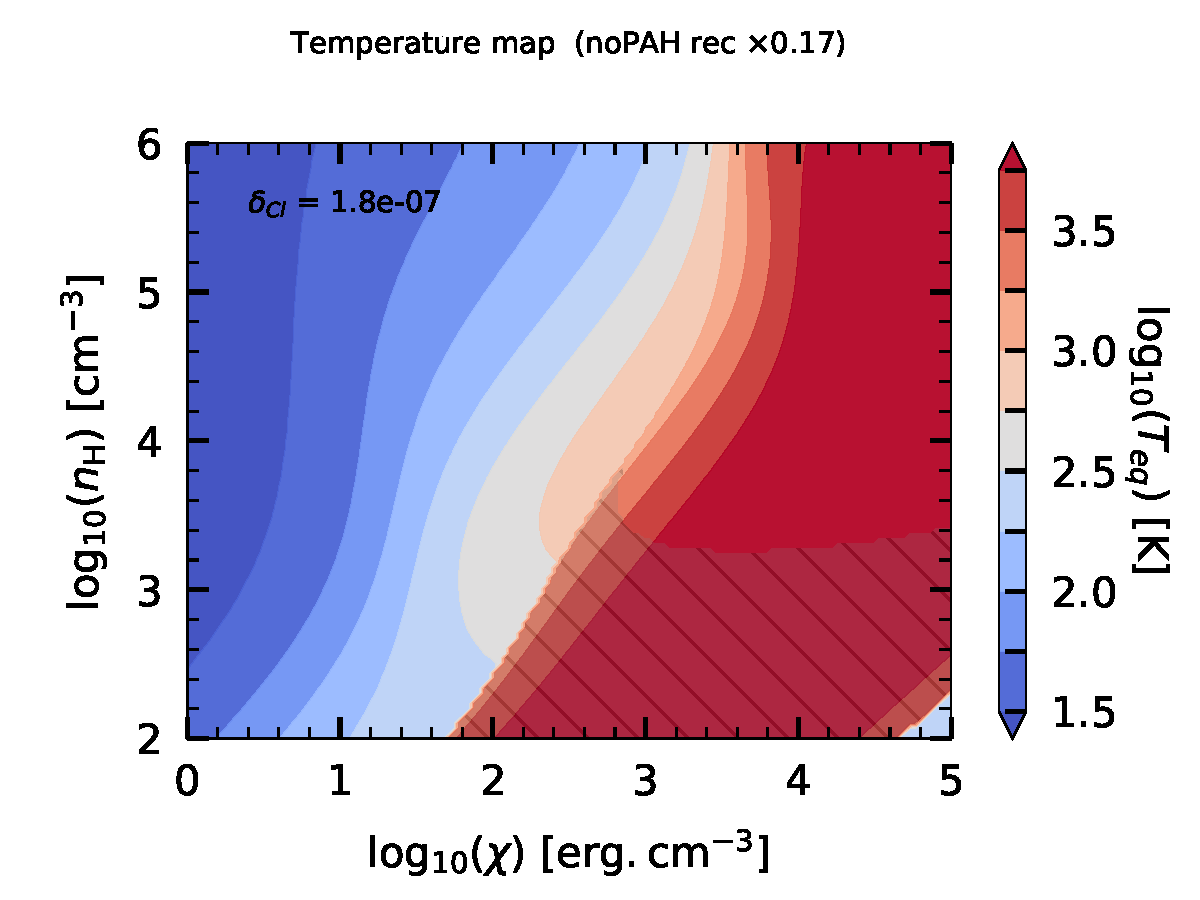
\includegraphics[trim = {0 0 0 1cm},clip,width=1\textwidth]{figure/Cl/gridModel/mapG0nHTeq_m6p7_imp_noPAH_3p0PE_OI_CII_ggr_elecrec_lyman_OI.pdf}
        \caption{avec chlore}
    \end{subfigure}
    ~ 
    \begin{subfigure}[t]{0.49\textwidth}
        \centering 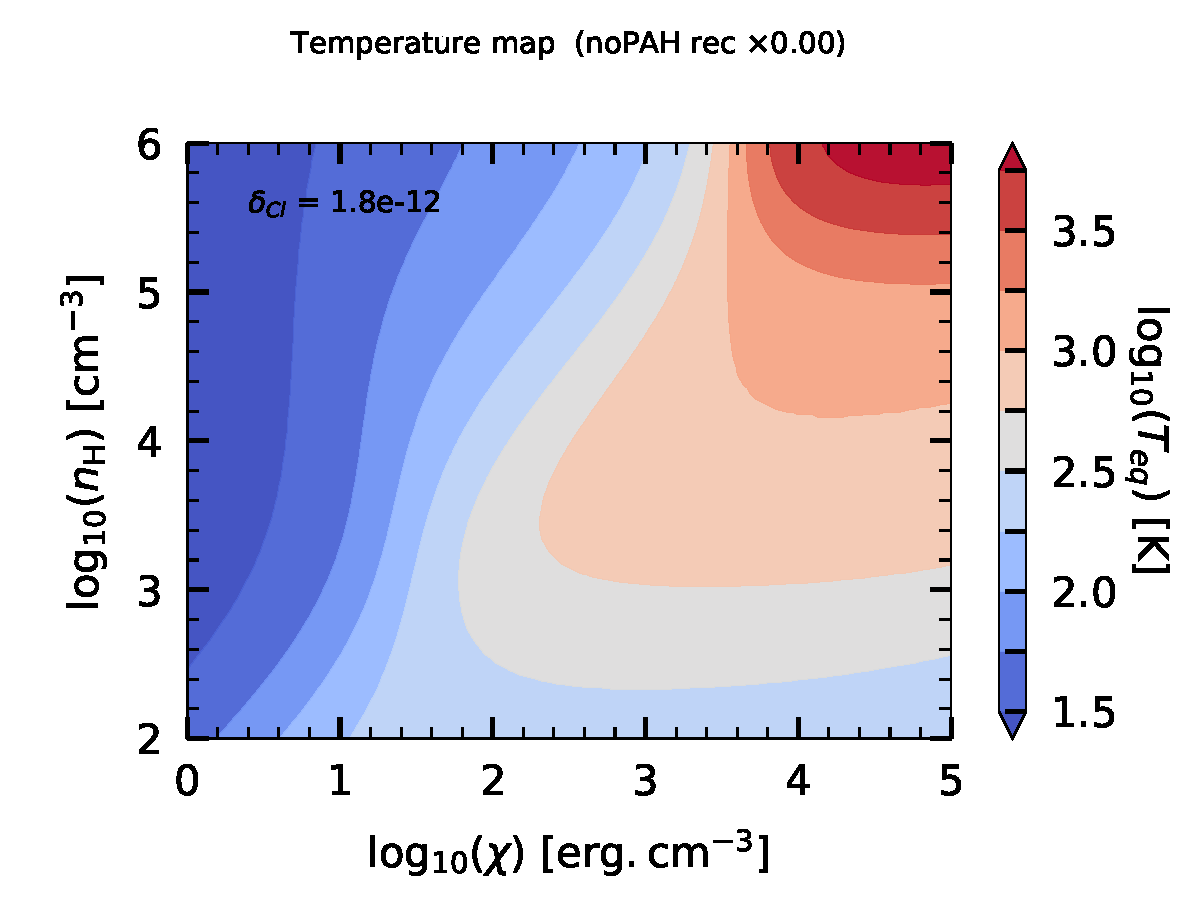
\includegraphics[trim = {0 0 0 1cm},clip,width=1\textwidth]{figure/Cl/gridModel/mapG0nHTeq_m11p7_exp_noPAH_3p0PE_OI_CII_ggr_elecrec_lyman_OI.pdf}
        \caption{sans chlore}
    \end{subfigure}
    \caption{Carte de température prédite par le modèle}
     \begin{minipage}{\textwidth} 
     La zone hachurée sur la figure (a) signifie qu'il existe plus d'une solution : au moins une solution stable et une solution instable.
     \label{fig:Cl:gridModel:Tba:noCl}
     \end{minipage}
    \label{fig:Cl:gridModel:Tba}
\end{figure}

Tout d'abord sur la figure \ref{fig:Cl:grid:Tba:noCl}, on remarque l'existence d'un point-selle en température vers $n_\mathrm{H}=10^3 \, \mathrm{cm}^{-3}$ et $\chi=10^3$ qui est absent de la figure \ref{fig:Cl:gridModel:Tba:noCl}. Une analyse de cette région montre que l'augmentation de l'intensité du champs de rayonnement $\chi$ dans les régions à basse densité accélère la recombinaison des électrons sur les grains qui la rend plus efficace que l'effet photoélectrique pur, ce qui diminue le chauffage net et donc la température du gaz. Les formules d'effet photoélectrique (eq \ref{eq:Rollig:pe}) et de recombinaisons des électrons sur les grains (eq \ref{eq:Rollig:rece}) reproduisent mal ce phénomène. Le modèle obtient dans ces régions des températures plus chaudes. \newline 

De plus, le code PDR calcule la température d'équilibre du gaz en cherchant par dichotomie les zéros de la fonction $\mathrm{T} \rightarrow (\Gamma - \Lambda)(\mathrm{T)}$. Rien n'assure que le code décèle toutes les solutions. Par exemple dans la figure \ref{fig:Cl:particulier:2}, le code ne trouve que la solution basse température alors qu'il existe une solution chaude proche de $9000$ K. Il peut arriver que le code saute d'une branche de solution à une autre comme c'est le cas sur le profil de température de la figure \ref{fig:Cl:firstprofil}. Une amélioration qui pourrait être faite au code est de le rendre capable de déceler deux solutions (s'il y en a) et de rester sur une même branche de solution à travers le nuage. \newline 

Enfin, l'absence de la prise en compte du $\mathrm{H}_2$ dans le modèle semi-analytique a un impact important sur la température car il chauffe par pompage UV les régions denses et refroidit par désexcitation collisionelle. On voit sur la figure \ref{fig:Cl:particulier:4} qui est un modèle dense ($n_\mathrm{H}=10^4 \, \mathrm{cm}^{-3}$, $\chi=10^{4.5}$) que l'effet photoélectrique est négligeable devant le chauffage par $\mathrm{H}_2$. 


\begin{figure}[!h]
    \centering
    \begin{subfigure}[t]{0.49\textwidth} % "0.49" donne ici la largeur de l'image
        \centering 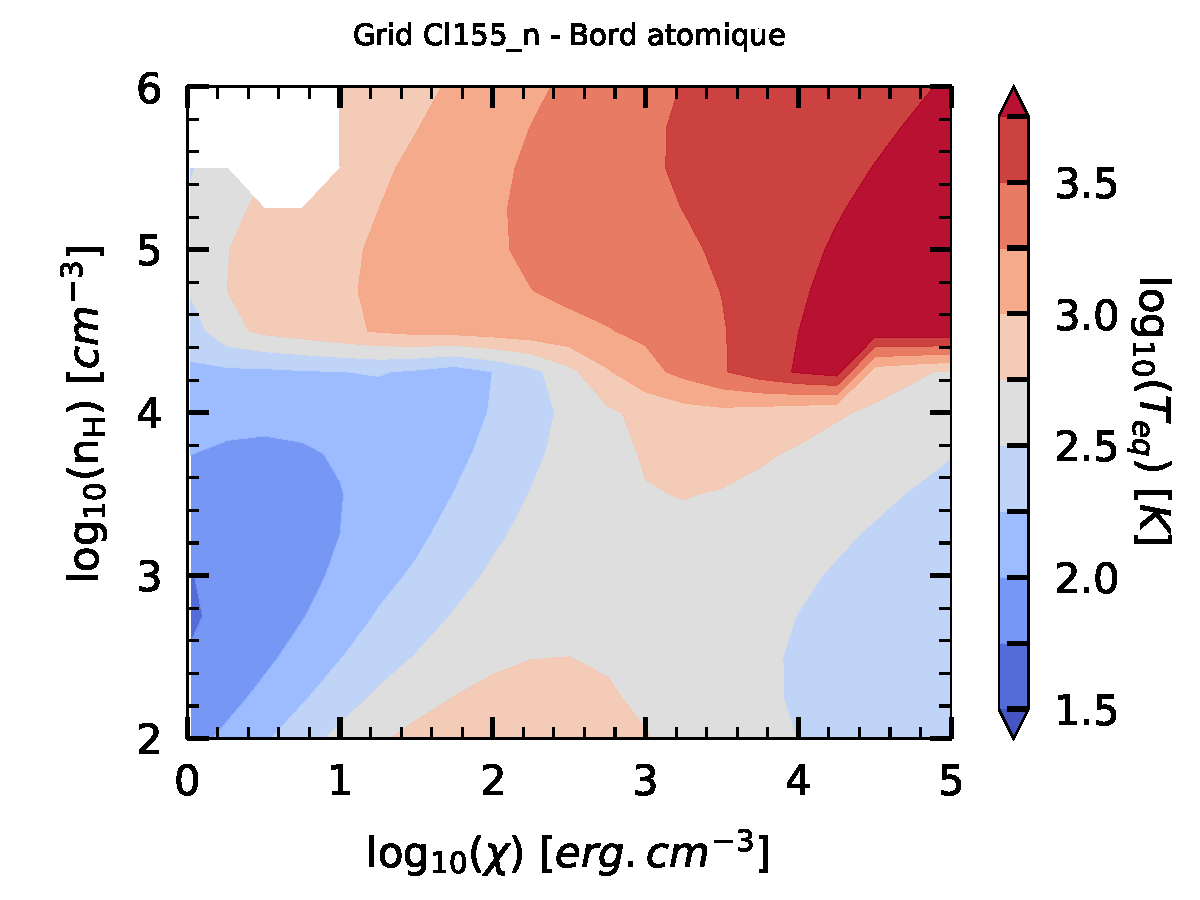
\includegraphics[trim = {0 0 0 1cm},clip,width=1\textwidth]{figure/Cl/gridCl155_n/mapTba.pdf}
        \caption{avec chlore}
    \end{subfigure}
    ~ 
    \begin{subfigure}[t]{0.49\textwidth}
        \centering 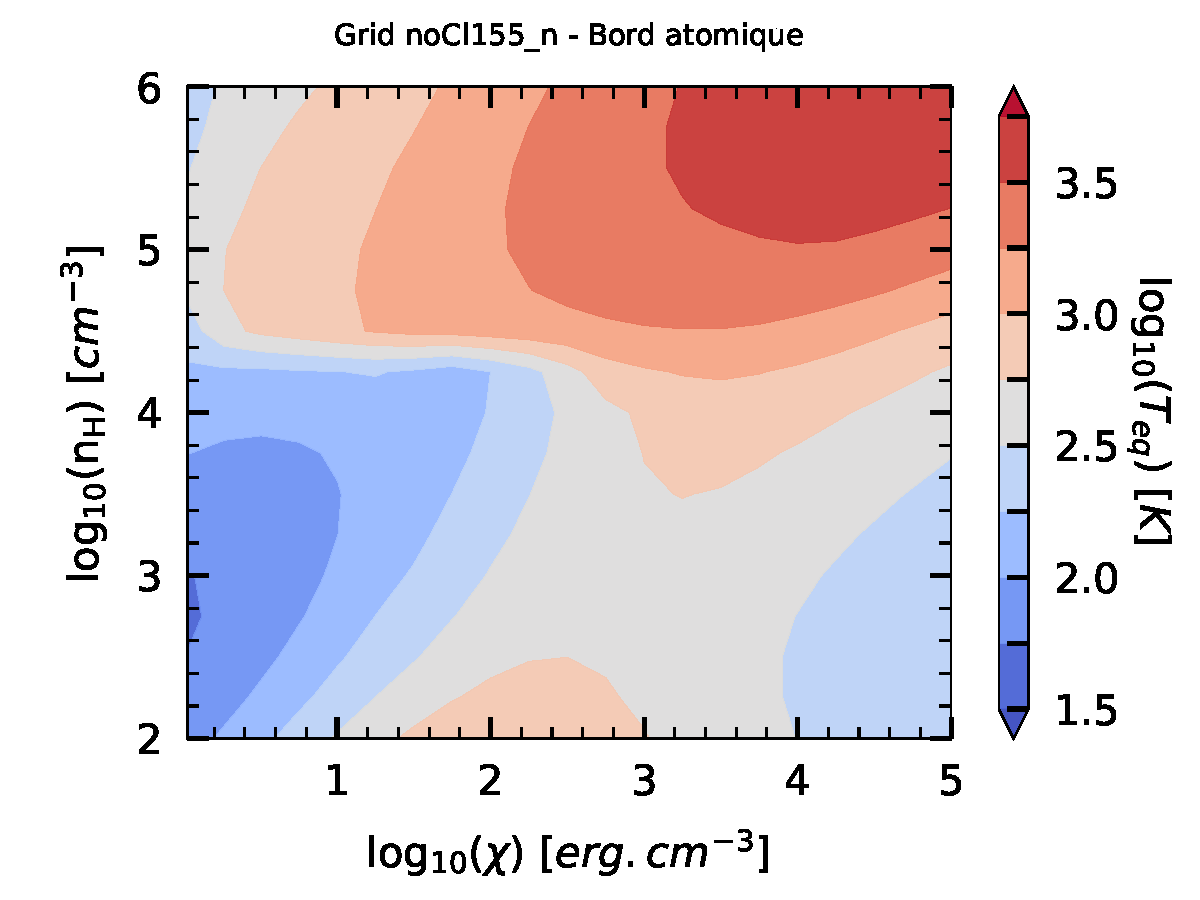
\includegraphics[trim = {0 0 0 1cm},clip,width=1\textwidth]{figure/Cl/gridnoCl155_n/mapTba.pdf}
        \caption{sans chlore}
        \label{fig:Cl:grid:Tba:noCl}
    \end{subfigure}
    \caption{Température en bord atomique de nuage calculé par le code PDR de Meudon}
    \label{fig:Cl:grid:Tba}
\end{figure}



% \begin{figure}[!h]
%     \centering
%     \begin{subfigure}[t]{0.49\textwidth} % "0.49" donne ici la largeur de l'image
%         \centering 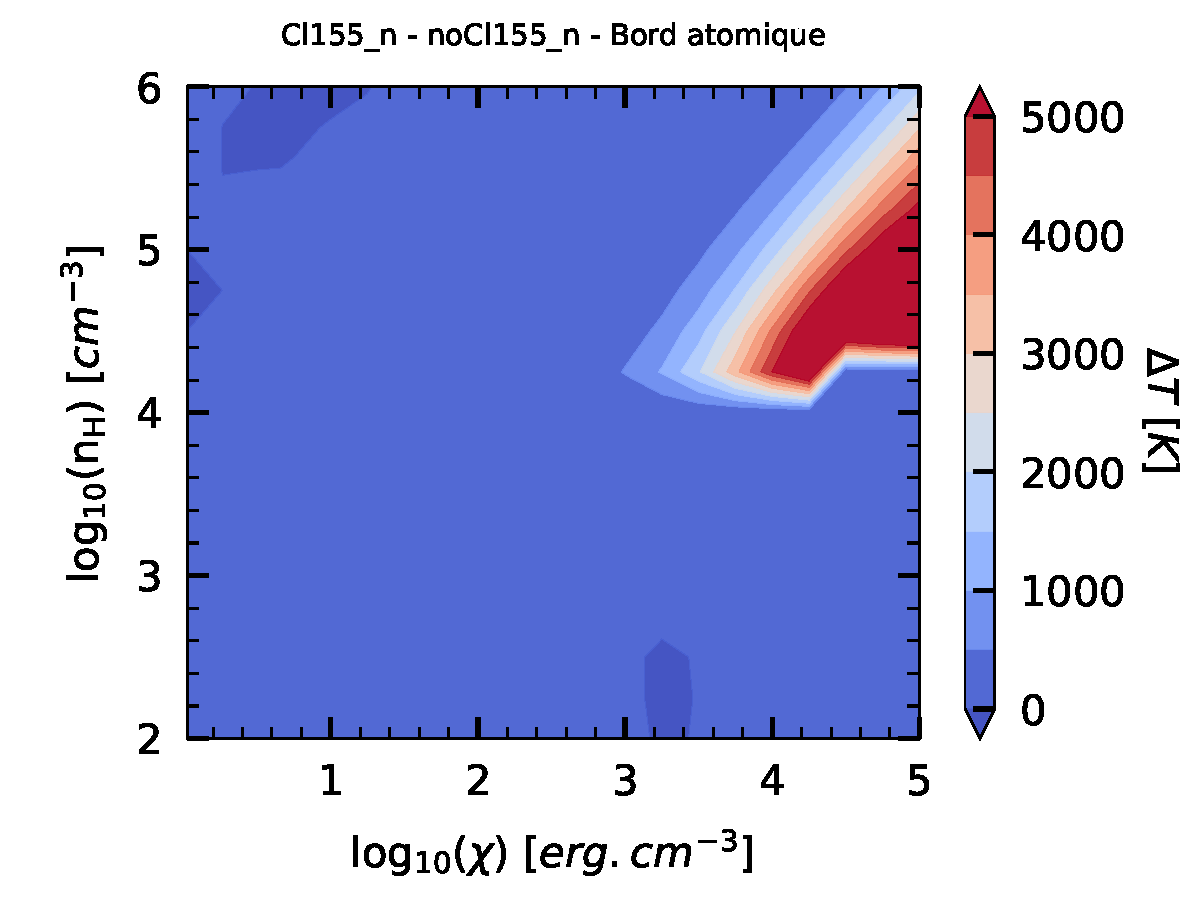
\includegraphics[trim = {0 0 0 1cm},clip,width=1\textwidth]{figure/Cl/gridCl155_n/mapTba_Cl155_n_noCl155_n.pdf}
%         \caption{différence de température en bord atomique}
%         \label{fig:Cl:grid:Tdiff}
%     \end{subfigure}
%     ~ 
%     \begin{subfigure}[t]{0.49\textwidth}
%         \centering 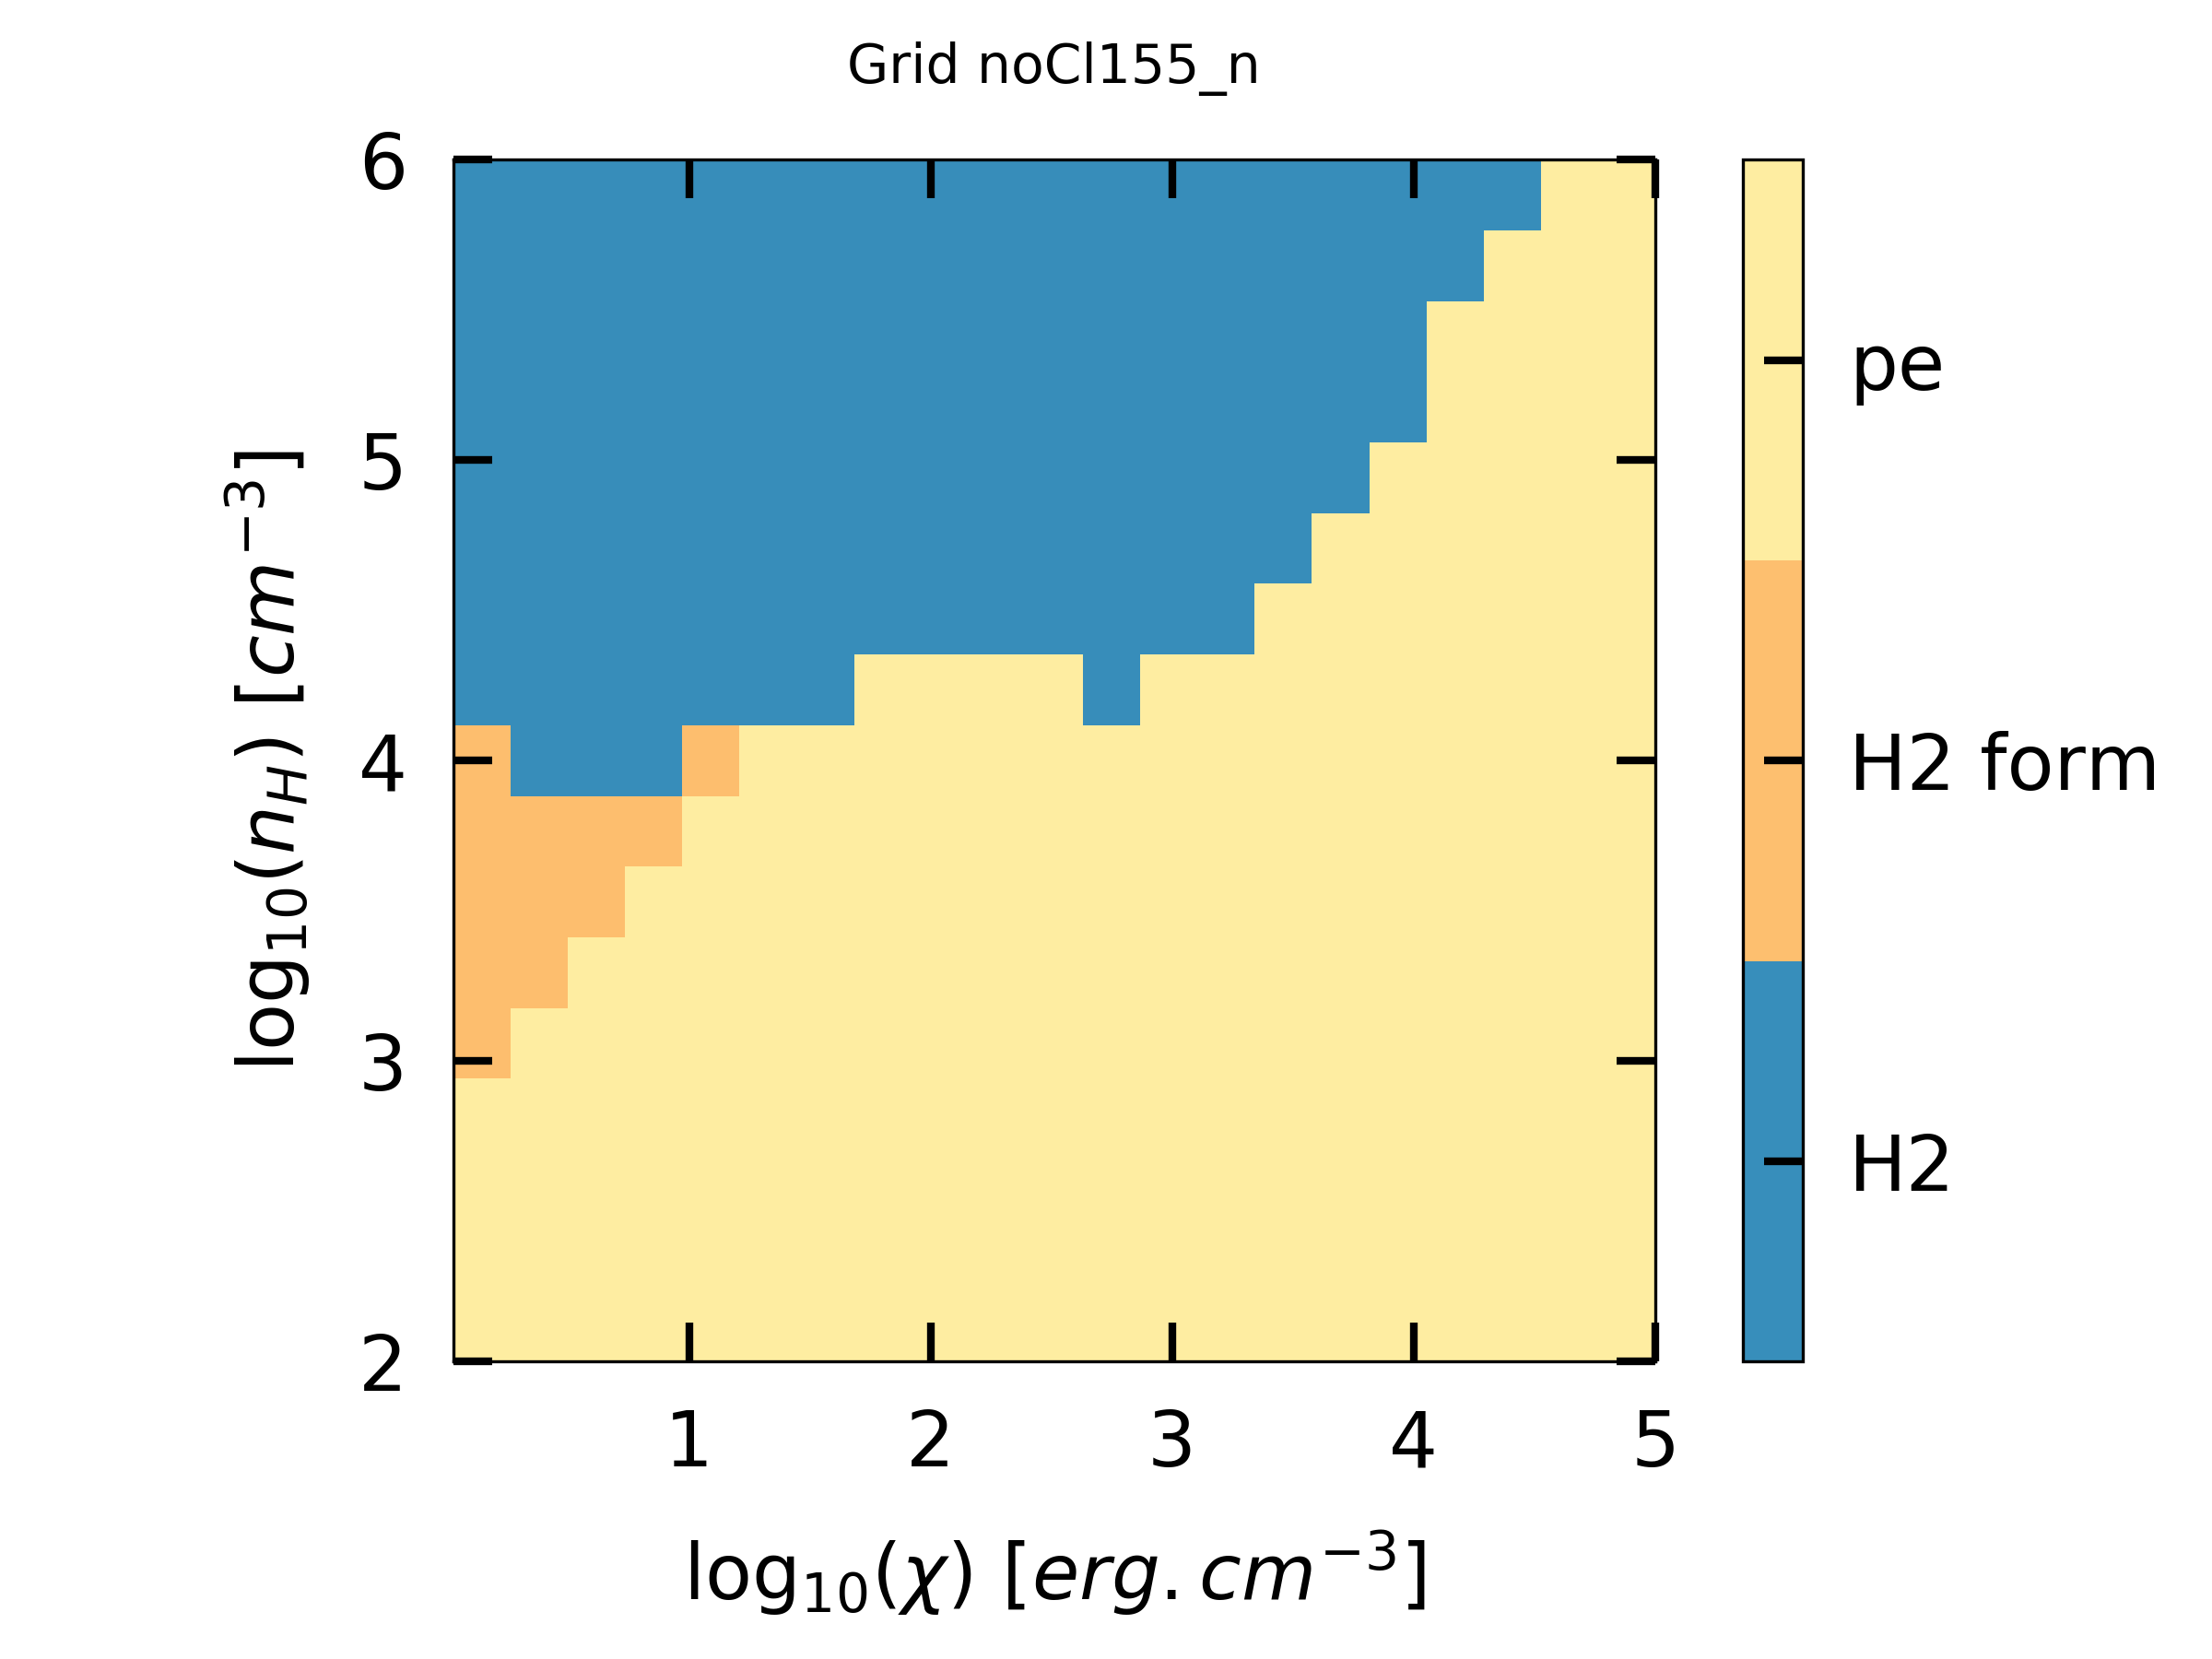
\includegraphics[trim = {0 0 0 1cm},clip,width=1\textwidth]{figure/Cl/gridnoCl155_n/mapGmax.png}
%         \caption{Processus de chauffage dominant en bord de nuage}
%         \label{fig:Cl:grid:Gmax}
%     \end{subfigure}
%     \caption{}
% \end{figure}


\begin{figure}[!h]
    \centering
    \begin{subfigure}[t]{0.49\textwidth} % "0.49" donne ici la largeur de l'image
        \centering 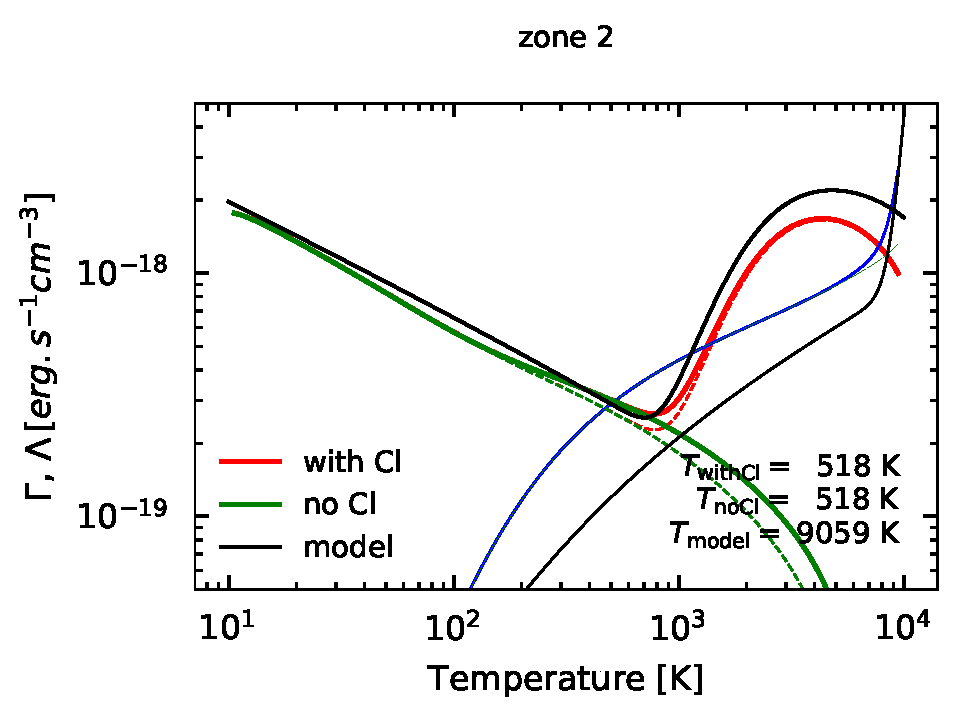
\includegraphics[trim = {0 0 0 1cm },clip,width=1\textwidth]{figure/Cl/particuliers/GCcomp_Cl_2.pdf}
        \caption{$n_\mathrm{H}=10^4 \, \mathrm{cm}^{-3}$, $\chi=10^{4.5}$}
        \label{fig:Cl:particulier:2}
    \end{subfigure}
    ~ 
    \begin{subfigure}[t]{0.49\textwidth}
        \centering 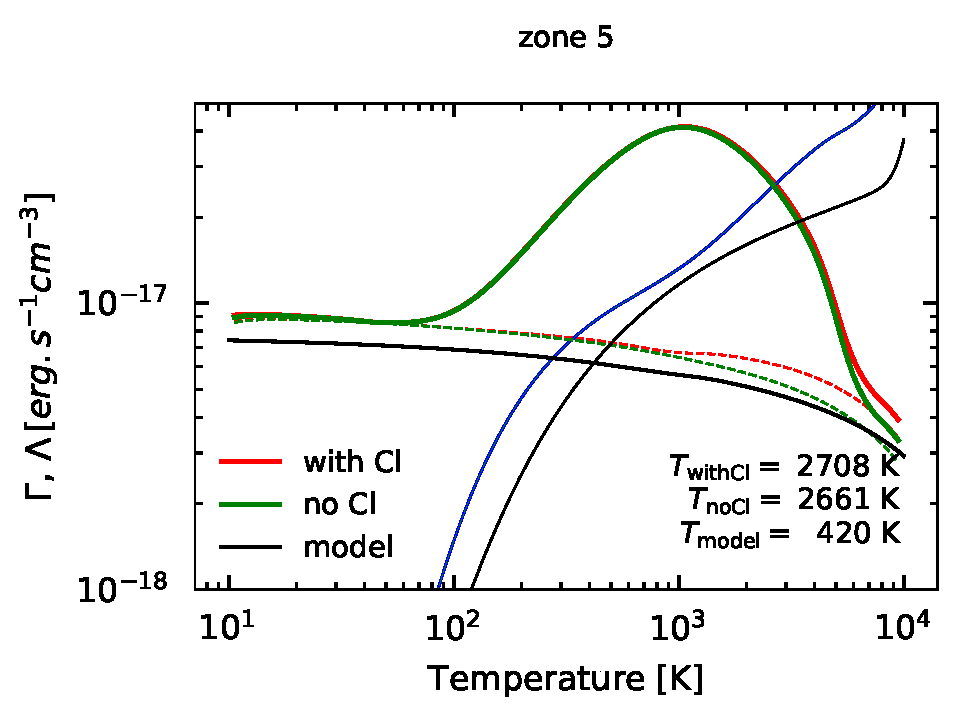
\includegraphics[trim = {0 0 0 1cm },clip,width=1\textwidth]{figure/Cl/particuliers/GCcomp_Cl_5.pdf}
        \caption{$n_\mathrm{H}=10^3 \, \mathrm{cm}^{-3}$, $\chi=10^3$}
        \label{fig:Cl:particulier:4}
    \end{subfigure}
    \caption{Courbes de chauffage et refroidissement, au bord atomique de nuage, de modèles résolus par le code PDR de Meudon. Mêmes règles de couleurs que dans la figure \ref{fig:Cl:modelPE:GC}.}
\end{figure}



%%%%%%%%%%%%%%%%%%%%%%%%%%%%%%%%%%%%%%%%%%%%%%%%%%%%%%%%%%%%%%%%%%%%%%%%%%%%%%%%%%%%%%%%%

\subsection{A la recherche d'observables}
\subsubsection{Détermination d'un traceur}

Nous avons pu prouver l'existence et expliquer le fonctionnement de l'instabilité provoquée par le chlore dans le bord atomique des PDR. Afin de l'observer, il est nécessaire de trouver les spectres d'émissions impactés par le chlore. \newline 

On choisit un modèle ($n_\mathrm{H}=10^5 \, \mathrm{cm}^{-3}$, $\chi=10^{4.5}$) dont le bord atomique devient nettement plus chaud lorsque l'on ajoute du chlore (figure \ref{fig:Cl:grid:Tba}). En traçant les spectres d'émission donnés par le code nous constatons que les raies $\mathrm{N}$, $\mathrm{N}^+$, $\mathrm{S}$, $\mathrm{Si}$ sont modifiées par la solution chaude (figure \ref{fig:Cl:gridModelEmiss:yes}). La présence du chlore augmente les raies du $\mathrm{N}$, $\mathrm{N}^+$ et $\mathrm{Si}$ d'un facteur 10 et du $\mathrm{S}$ d'un facteur 100. Bien que le chlore intensifient de manière importante les raies d'émissions, il y existe un seuil d'observabilité, de l'ordre de $10^{-6} \ \mathrm{erg}\,\mathrm{cm}^{-2}\,\mathrm{s}^{-1}$, au dessus duquel les raies sont expérimentalement mesurables. Par conséquent on peut considérer seulement certaines raies du spectre de $\mathrm{N}$. En revanche, les raies du $\mathrm{CS}$, $\mathrm{H}_2\mathrm{O}$, $\mathrm{H}_2$, ne sont pas affectées par la présence de chlore dans le nuage (figure \ref{fig:Cl:gridModelEmiss:no}) car il agit dans la zone atomique du nuage où les molécules ne sont pas formés. \newline

\begin{figure}[!h]
    \centering
    \begin{subfigure}[t]{0.49\textwidth} % "0.49" donne ici la largeur de l'image
        \centering 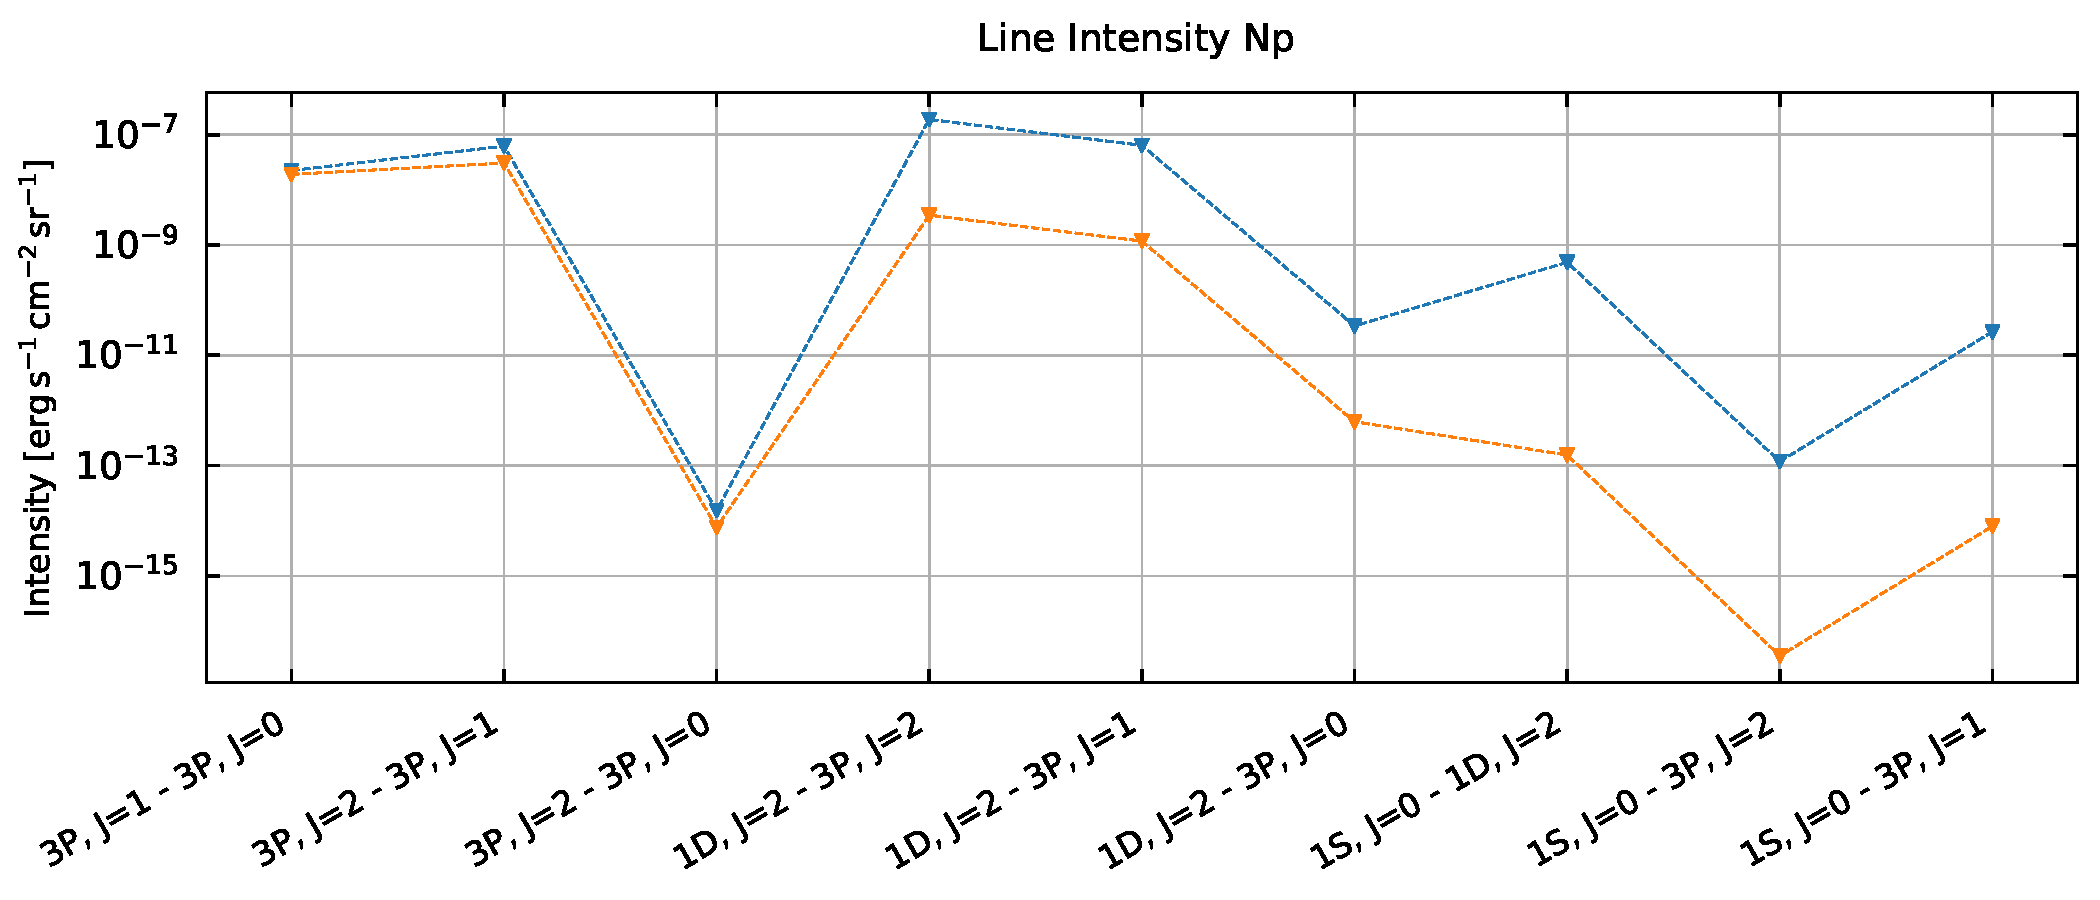
\includegraphics[trim = {0 0 0 1cm},clip,width=1\textwidth]{figure/Cl/gridModelEmiss/I_comp_Np.pdf}
        \caption{$\mathrm{N}^+$}
    \end{subfigure}
    ~ 
   \begin{subfigure}[t]{0.49\textwidth} % "0.49" donne ici la largeur de l'image
        \centering 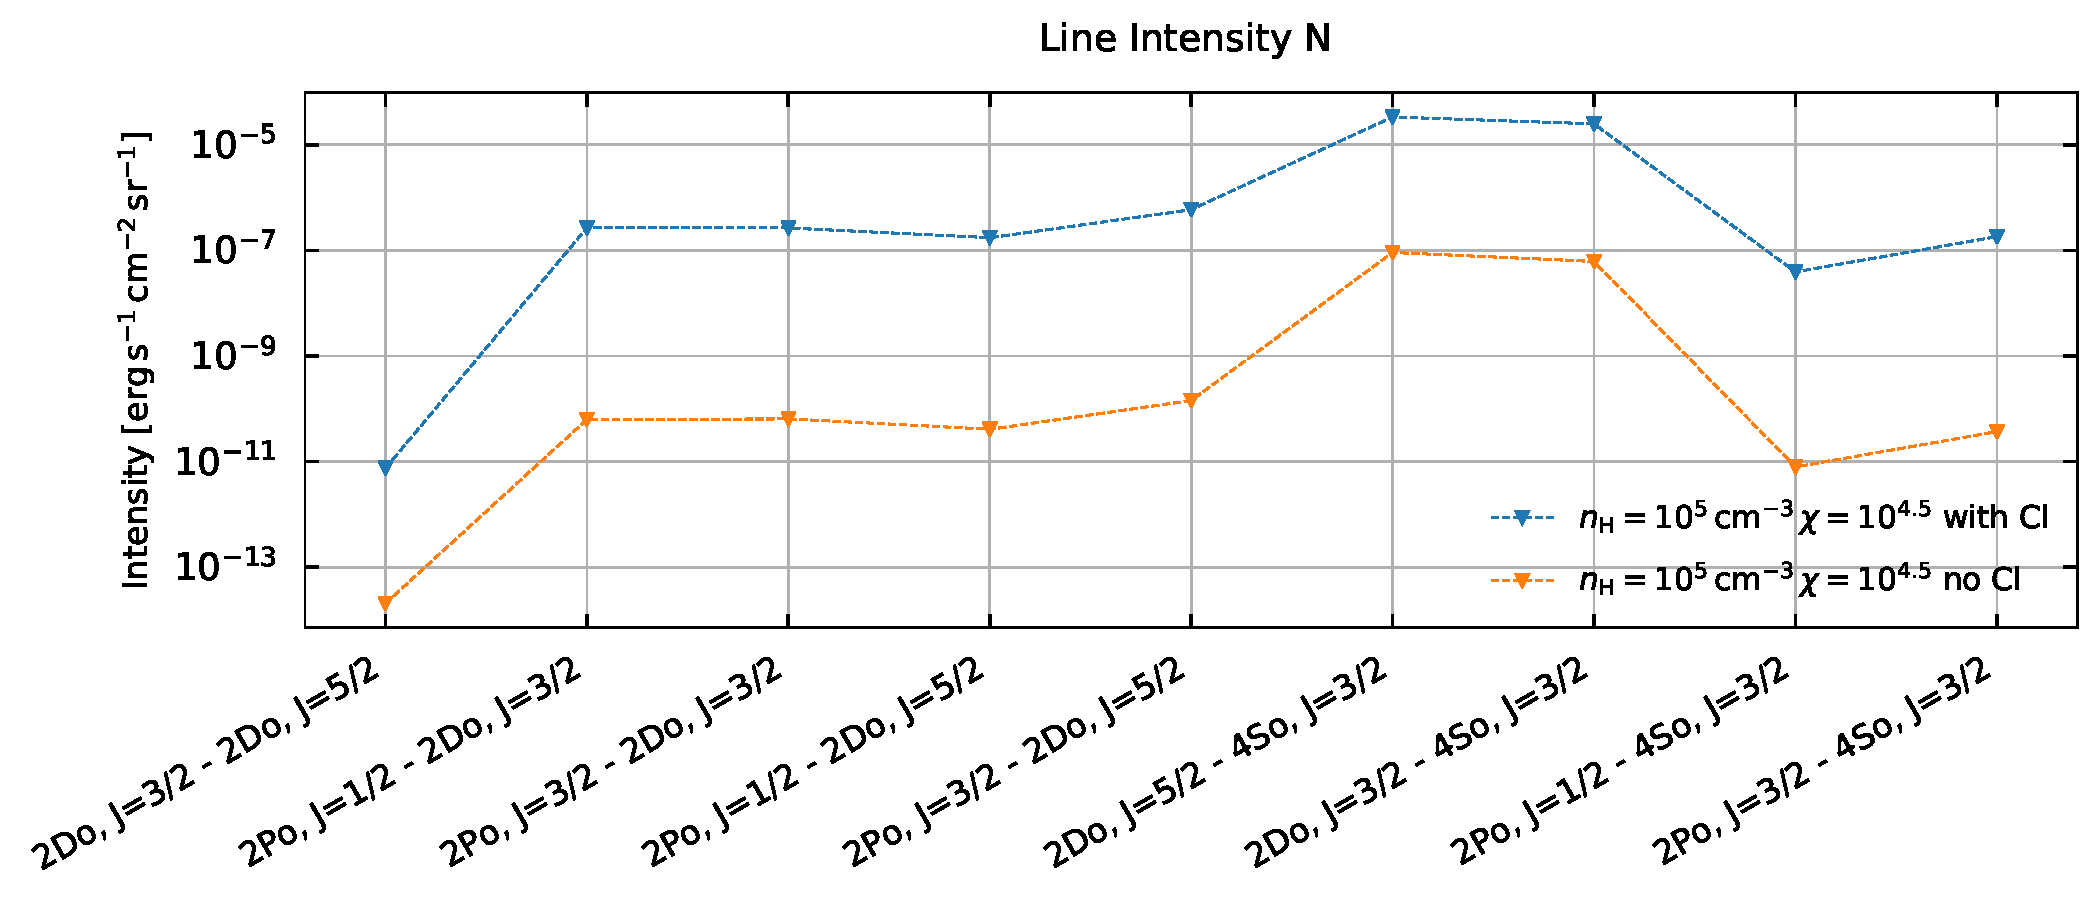
\includegraphics[trim = {0 0 0 1cm},clip,width=1\textwidth]{figure/Cl/gridModelEmiss/I_comp_N.pdf}
        \caption{$\mathrm{N}$}
    \end{subfigure}
    
    \begin{subfigure}[t]{0.49\textwidth} % "0.49" donne ici la largeur de l'image
        \centering 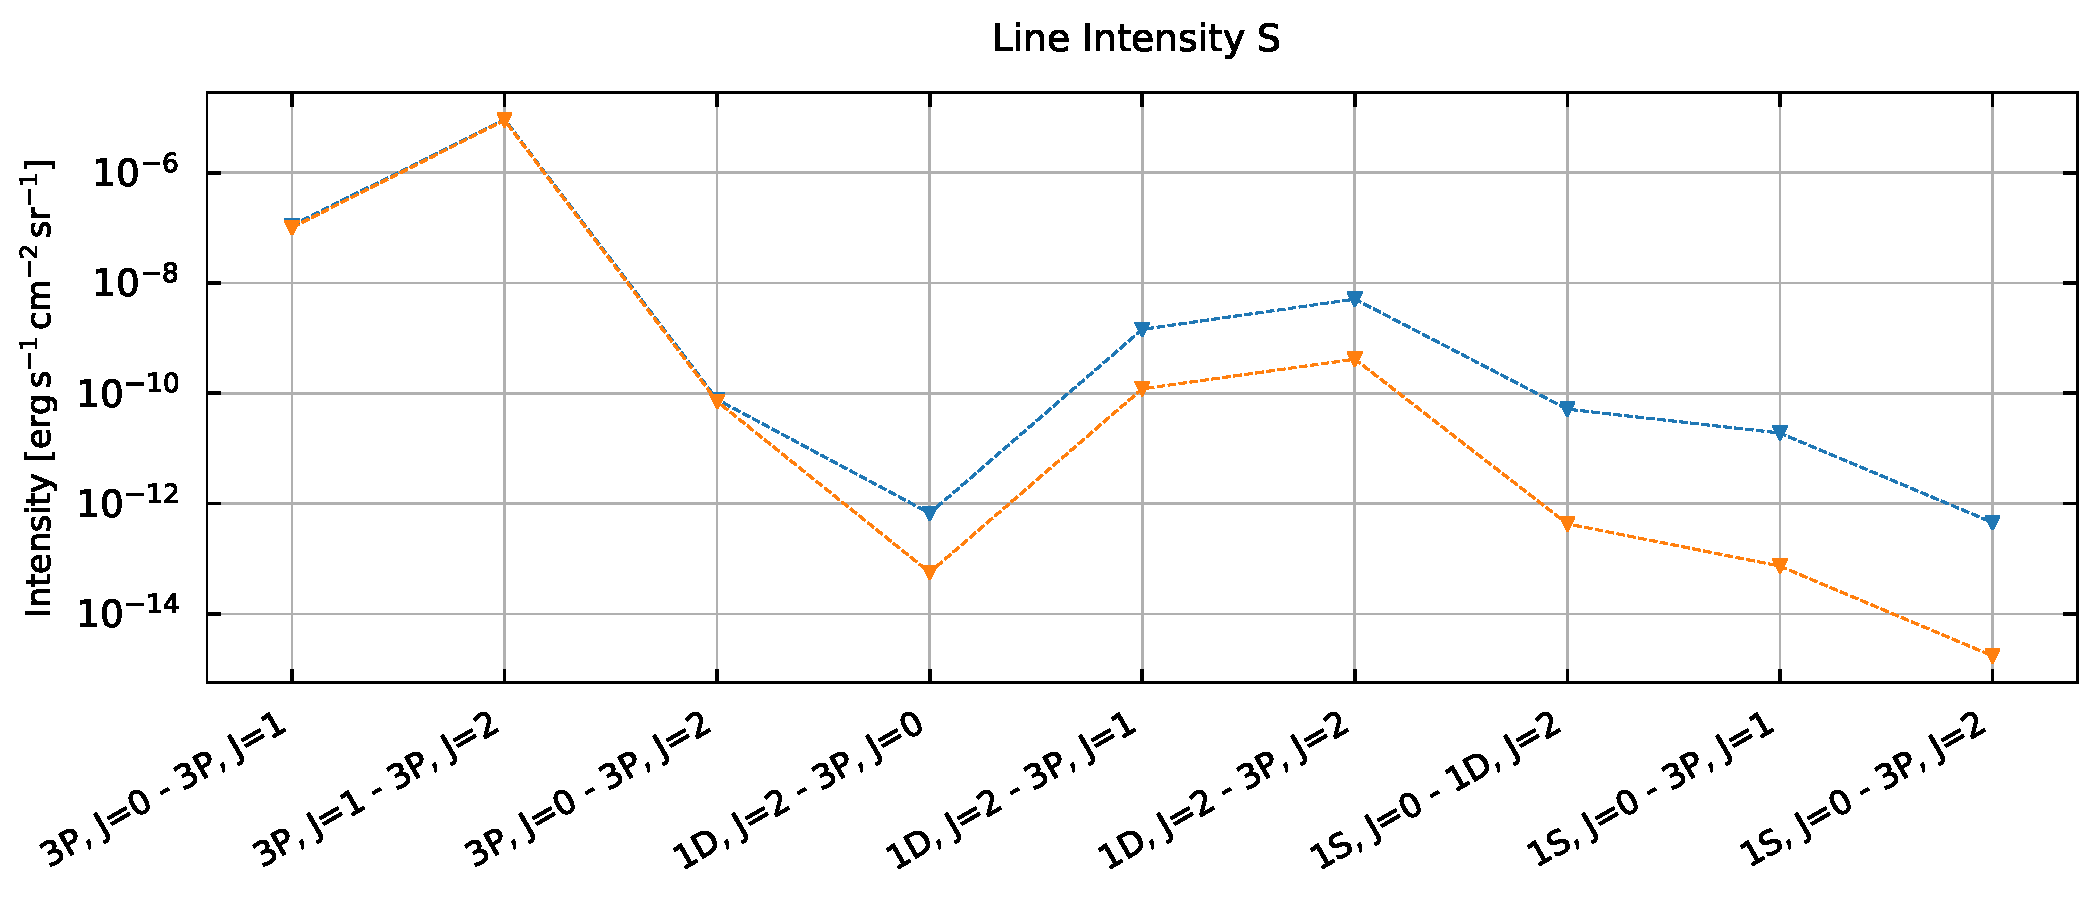
\includegraphics[trim = {0 0 0 1cm},clip,width=1\textwidth]{figure/Cl/gridModelEmiss/I_comp_S.pdf}
        \caption{$\mathrm{S}$}
    \end{subfigure}
    ~
    \begin{subfigure}[t]{0.49\textwidth} % "0.49" donne ici la largeur de l'image
        \centering 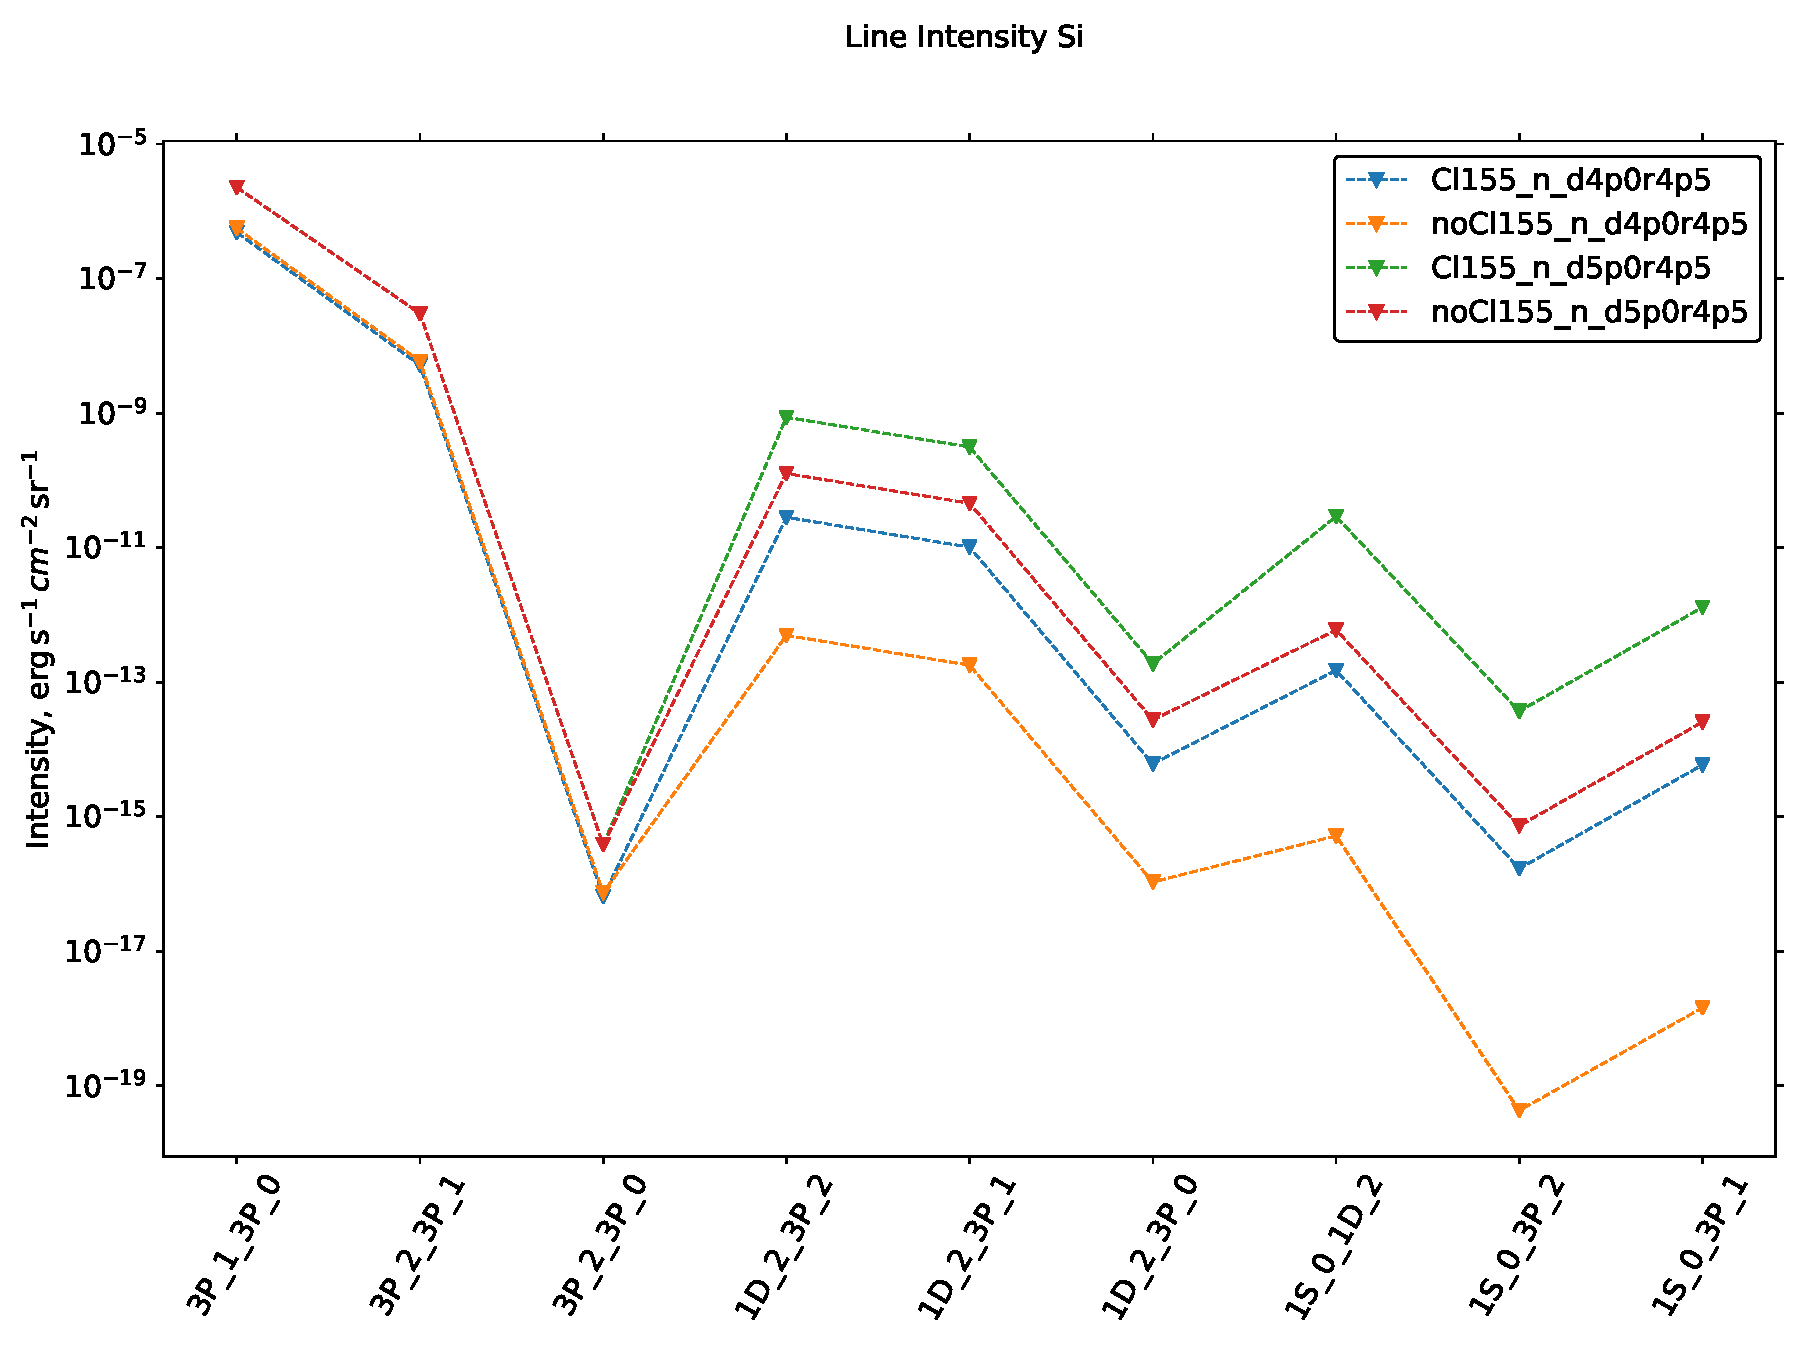
\includegraphics[trim = {0 0 0 1cm},clip,width=1\textwidth]{figure/Cl/gridModelEmiss/I_comp_Si.pdf}
        \caption{$\mathrm{Si}$}
    \end{subfigure}
    
    \caption{Diagramme d'intensité des traceurs modifiés par l'ajout du chlore.}
    \begin{minipage}{\textwidth}
    Les traits en bleue et orange sont les modèles $n_\mathrm{H}=10^5 \, \mathrm{cm}^{-3}$ et $\chi=10^{4.5}$ avec et sans le chlore (respectivement). Ces spectres sont affichés en plus grande taille dans l'annexe.
    \end{minipage}
    \label{fig:Cl:gridModelEmiss:yes}
\end{figure}

% \subsubsection{Profils de densités des traceurs}



\subsubsection{Choix de la raie $[\mathrm{N}]\,5200 \mathrm{A}$}

On choisit la raie la plus intense du spectre d'émission de $\mathrm{N}$ qui est la transition $\mathrm{Eu}=2\mathrm{D}^\mathrm{0}_{5/2} \rightarrow \mathrm{El}=4\mathrm{S}^\mathrm{0}_{3/2}$ correspondant à la longueur d'onde $5200 \AA$. Cette raie est dans le domaine du visible et pourrait être observé depuis la Terre par MUSE. \newline 

La figure \ref{fig:Cl:gridModelEmiss:N} représente le rapport d'intensité de la raie $[\mathrm{N}]\,5200 \mathrm{A}$ des grilles de modèle contenant du chlore ou ne contenant pas de chlore. On constate que les régions dont les bords atomiques qui subissent l'emballement de l'effet photoélectrique (figure \ref{fig:Cl:grid:Tba}) ont des intensités de raies jusqu'à $10^6$ fois plus grande. Tenter d'observer cette raie permettrait à priori de déterminer les bords atomiques des PDR chauffés par le chlore. \newline 

Il est cependant quasi impossible de l'observer car l'émission du $\mathrm{N}$ dans la partie atomique sera masquée par les émissions de l'azote atomique situé avant le front d'ionisation de l'hydrogène. En effet, le potentiel d'ionisation de l'azote est $14.6\,\mathrm{eV}$ qui est plus grand que celui de l'hydrogène ($13.6\,\mathrm{eV}$) ce qui signifie que le front d'ionisation de l'azote est devant celui de l'hydrogène. La raie de l'azote est produite par des excitations collisionnelles (avec $\mathrm{H}$,$\mathrm{H}^+$ $\mathrm{H}_2$, $\mathrm{He}$ et $e^-$ qui sont les espèces majoritaires dans le nuage) suivies d'émissions spontanées. La fraction électronique dans la partie atomique est de $10^{-3}$ alors qu'elle est de 1 dans la partie ionisé ce qui signifie que l'augmentation de l'intensité de la raie que l'on a observé est négligeable devant les émissions de $\mathrm{N}$ dans la partie ionisé du nuage.\newline

Il est donc nécessaire de déterminer des traceurs qui ont des potentiels de ionisations inférieurs à celui de l'hydrogène et émettent dans le bord atomique du nuage. 

\begin{figure}[!h]
    \centering 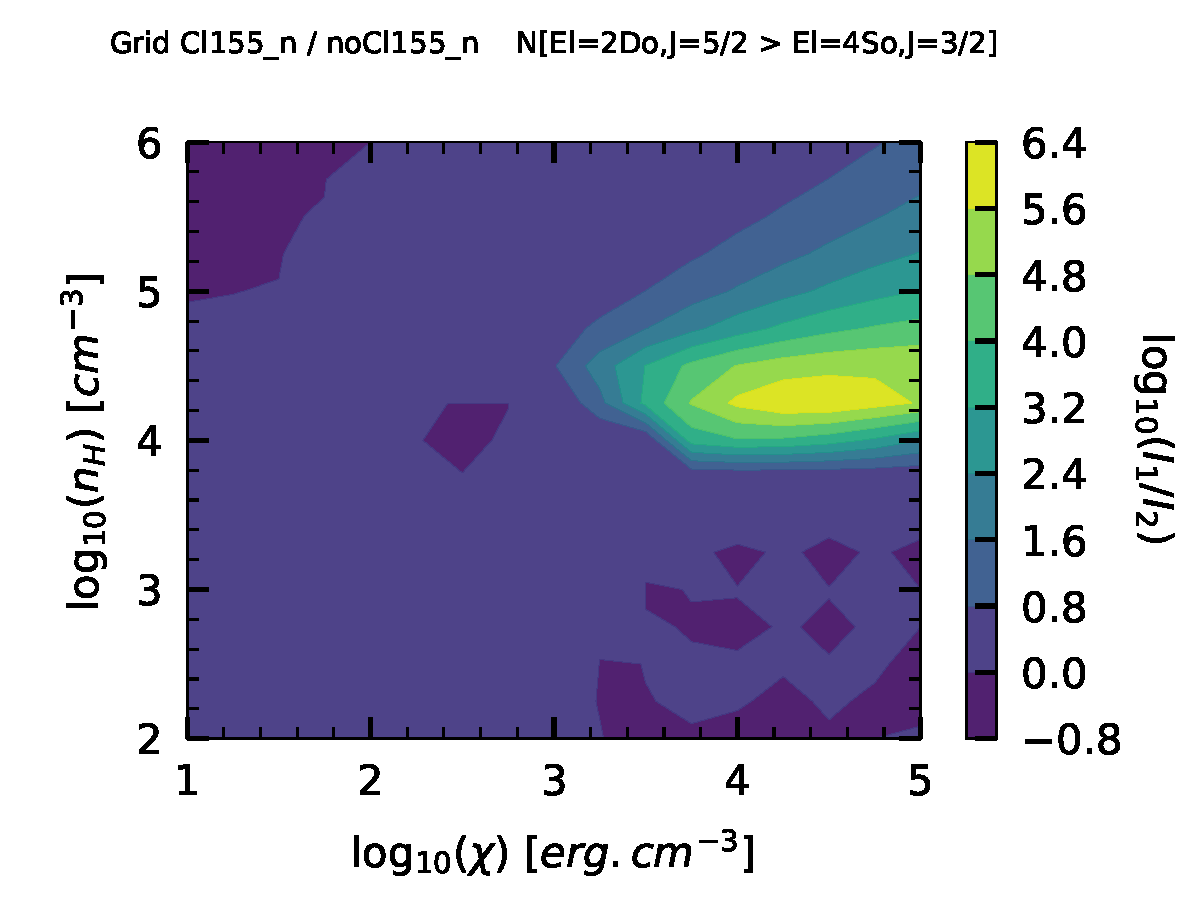
\includegraphics[trim = {0 0 0 1cm},clip,width=0.5\textwidth]{figure/Cl/gridModelEmiss/map_Cl155_n_noCl155_nI_N.pdf}
    \caption{Rapport des intensités de grilles de modèles contenant, ou non, du chlore a refaire + schéma des front de ionisations + aller jusqu'à $10^0$}
    \label{fig:Cl:gridModelEmiss:N}
\end{figure}





%%%%%%%%%%%%%%%%%%%%%%%%%%%%%%%%%%%%%%%%%%%%%%%%%%%%%%%%%%%%%%%%%%%%%%%%%%%%%%%%%%%%%%%%%%%%%%%

% \subsection{Bonus}
% \subsubsection{Chauffage à l'entrée du nuage moléculaire}

% Il arrive qu'en entrée du nuage moléculaire, la température du gaz augmente de manière irrégulière. Dans cette région, l'effet photoélectrique devient encore plus efficace en raison de l'augmentation de la fraction électronique du nuage. La recombinaison sur les grains est d'autant plus rapide que la fraction électronique est grande. 

% % Dans cette région du nuage, le $\mathrm{H}_2$ se forme principalement sut les grains mais aussi par l'association radiative de l'hydrogène :

% % \begin{equation}
% %     \begin{array}{lccccclr}
% %       \mathrm{H}  & + & e^- & \rightarrow & \mathrm{H}^{-} & + & h\nu &  \\
% %     \end{array}
% % \end{equation}

% % avec un coefficient de réaction $k(T) = 1.9\, 10^{-16} \big(\frac{T}{100}\big)^{0.67} \, \mathrm{cm}^3\mathrm{s}^{-1}$, suivi d'un détachement associatif :

% % \begin{equation}
% %     \begin{array}{lcccccclr}
% %       \mathrm{H}  & + &  \mathrm{H}^- & \rightarrow & \mathrm{H}_2 & + & e^- & + & KE\\
% %     \end{array}
% % \end{equation}

% % ou $\xi = 2.4\, 10^{-7} G_0 \, \mathrm{s}^{-1}$. 

% On a remarqué que pour une PDR avec $n_\mathrm{H} = 10^{3.5} \, \mathrm{cm}^{-3}$ et $\chi = 10^{4.5}$, la température augmentait en pic avant le nuage moléculaire (figure \ref{fig:H2:recomb:profilH}). On cherche à comprendre quel phénomène est à l'origine de l'augmentation de la température ? Pourquoi le taux de H2 diminue t il en même temps ? Pourquoi prendre en compte les nouveaux taux de collisions accentue ce phénomène ? Qu'est ce qui provoque la monté ? Pourquoi ça s'arrête : lorsque la température du gaz est trop élevé, les états ro-vibrationelles de H2 sont remplis et se desexcitent en émettant des photons. On le voit sur la figure \ref{fig:H2:recomb:profilH} ou le chauffage par H2 cessent de chauffer.

% \begin{figure}[!htbp]
%     \centering
%     \begin{subfigure}[t]{0.49\textwidth} % "0.49" donne ici la largeur de l'image
%         \centering 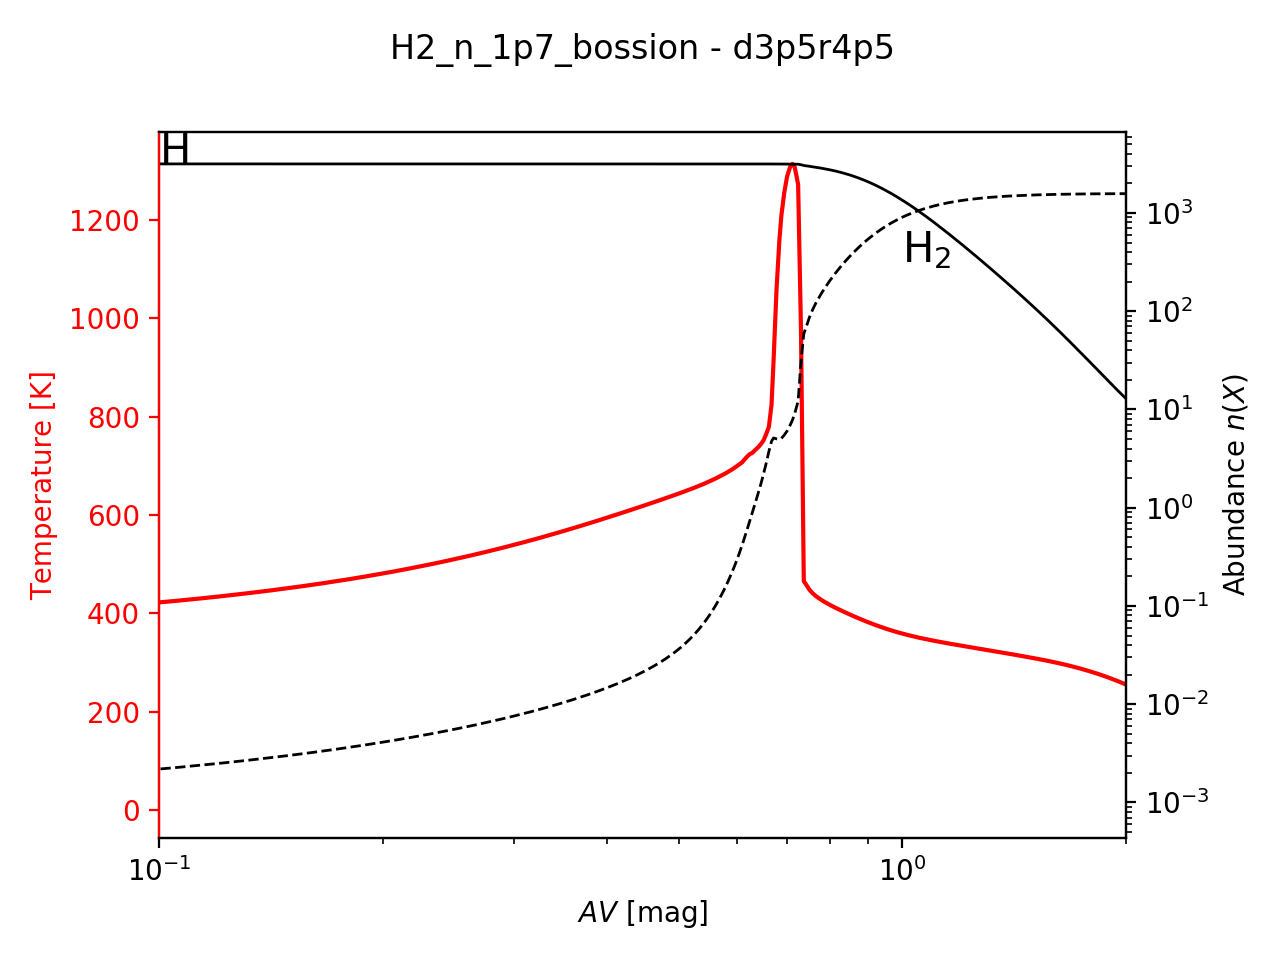
\includegraphics[trim = {0 0 0 1cm},clip,width=1\textwidth]{figure/H2/rec_elec/H2_n_1p7_bossion_d3p5r4p5_H.png}
%         \caption{}
%     \end{subfigure}
%     ~ 
%     \begin{subfigure}[t]{0.49\textwidth} % "0.49" donne ici la largeur de l'image
%         \centering 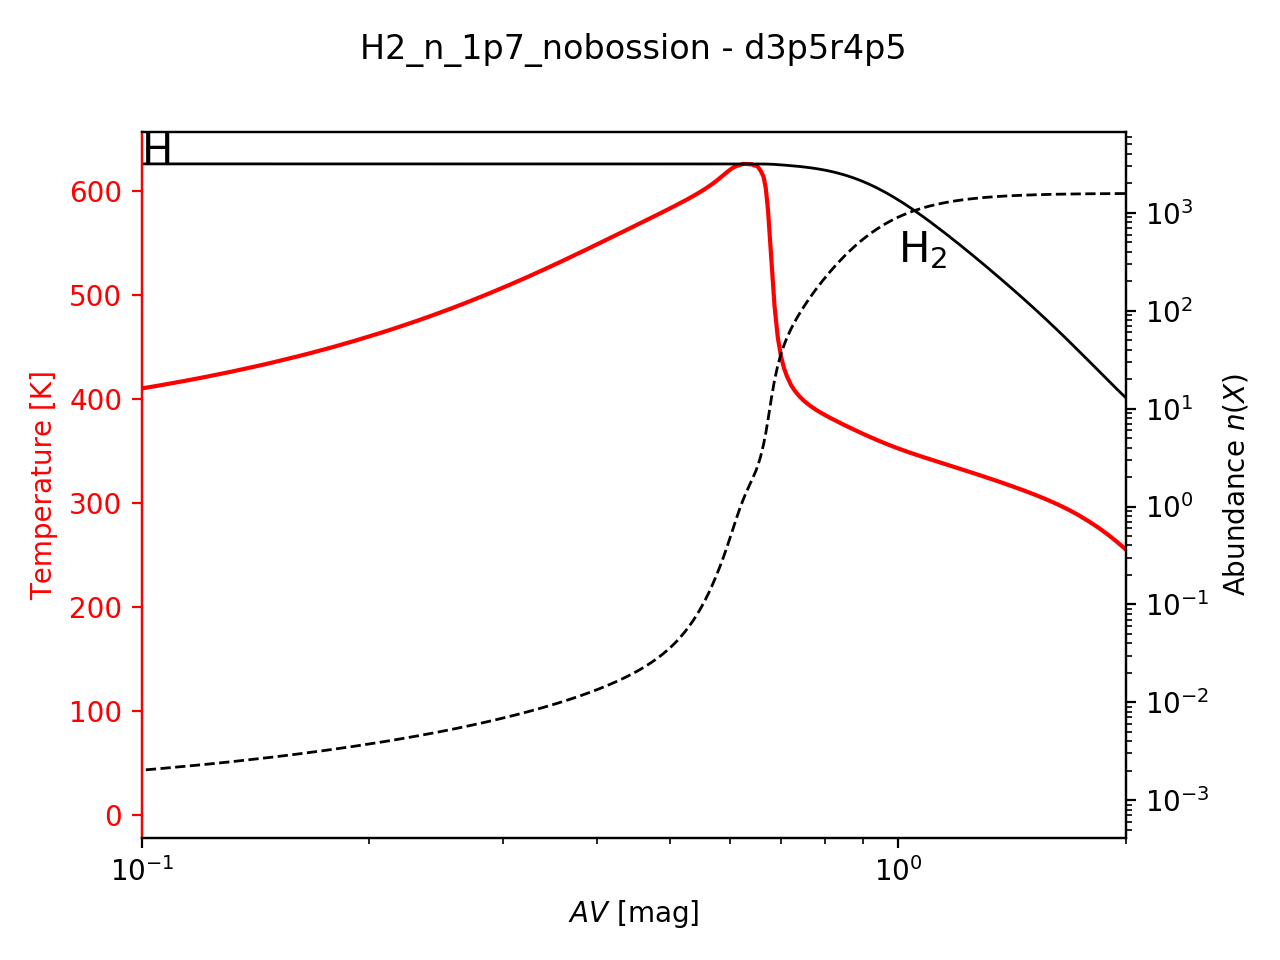
\includegraphics[trim = {0 0 0 1cm},clip,width=1\textwidth]{figure/H2/rec_elec/H2_n_1p7_nobossion_d3p5r4p5_H.png}
%         \caption{}
%     \end{subfigure}
    
%     \caption{Profil de température et de densités de $\mathrm{H}$ et $\mathrm{H}_2$. A l'entrée du nuage la température augmente accompagné d'une légère diminution de la densité de $\mathrm{H}_2$. Cet effet est accentué sur (a) qui prend en compte les nouveaux taux de collision de $\mathrm{H}_2$. }
%     \label{fig:H2:recomb:profilH}
% \end{figure}
    
% \begin{figure}[!htbp]
%     \centering
%     \begin{subfigure}[t]{0.49\textwidth} % "0.49" donne ici la largeur de l'image
%         \centering 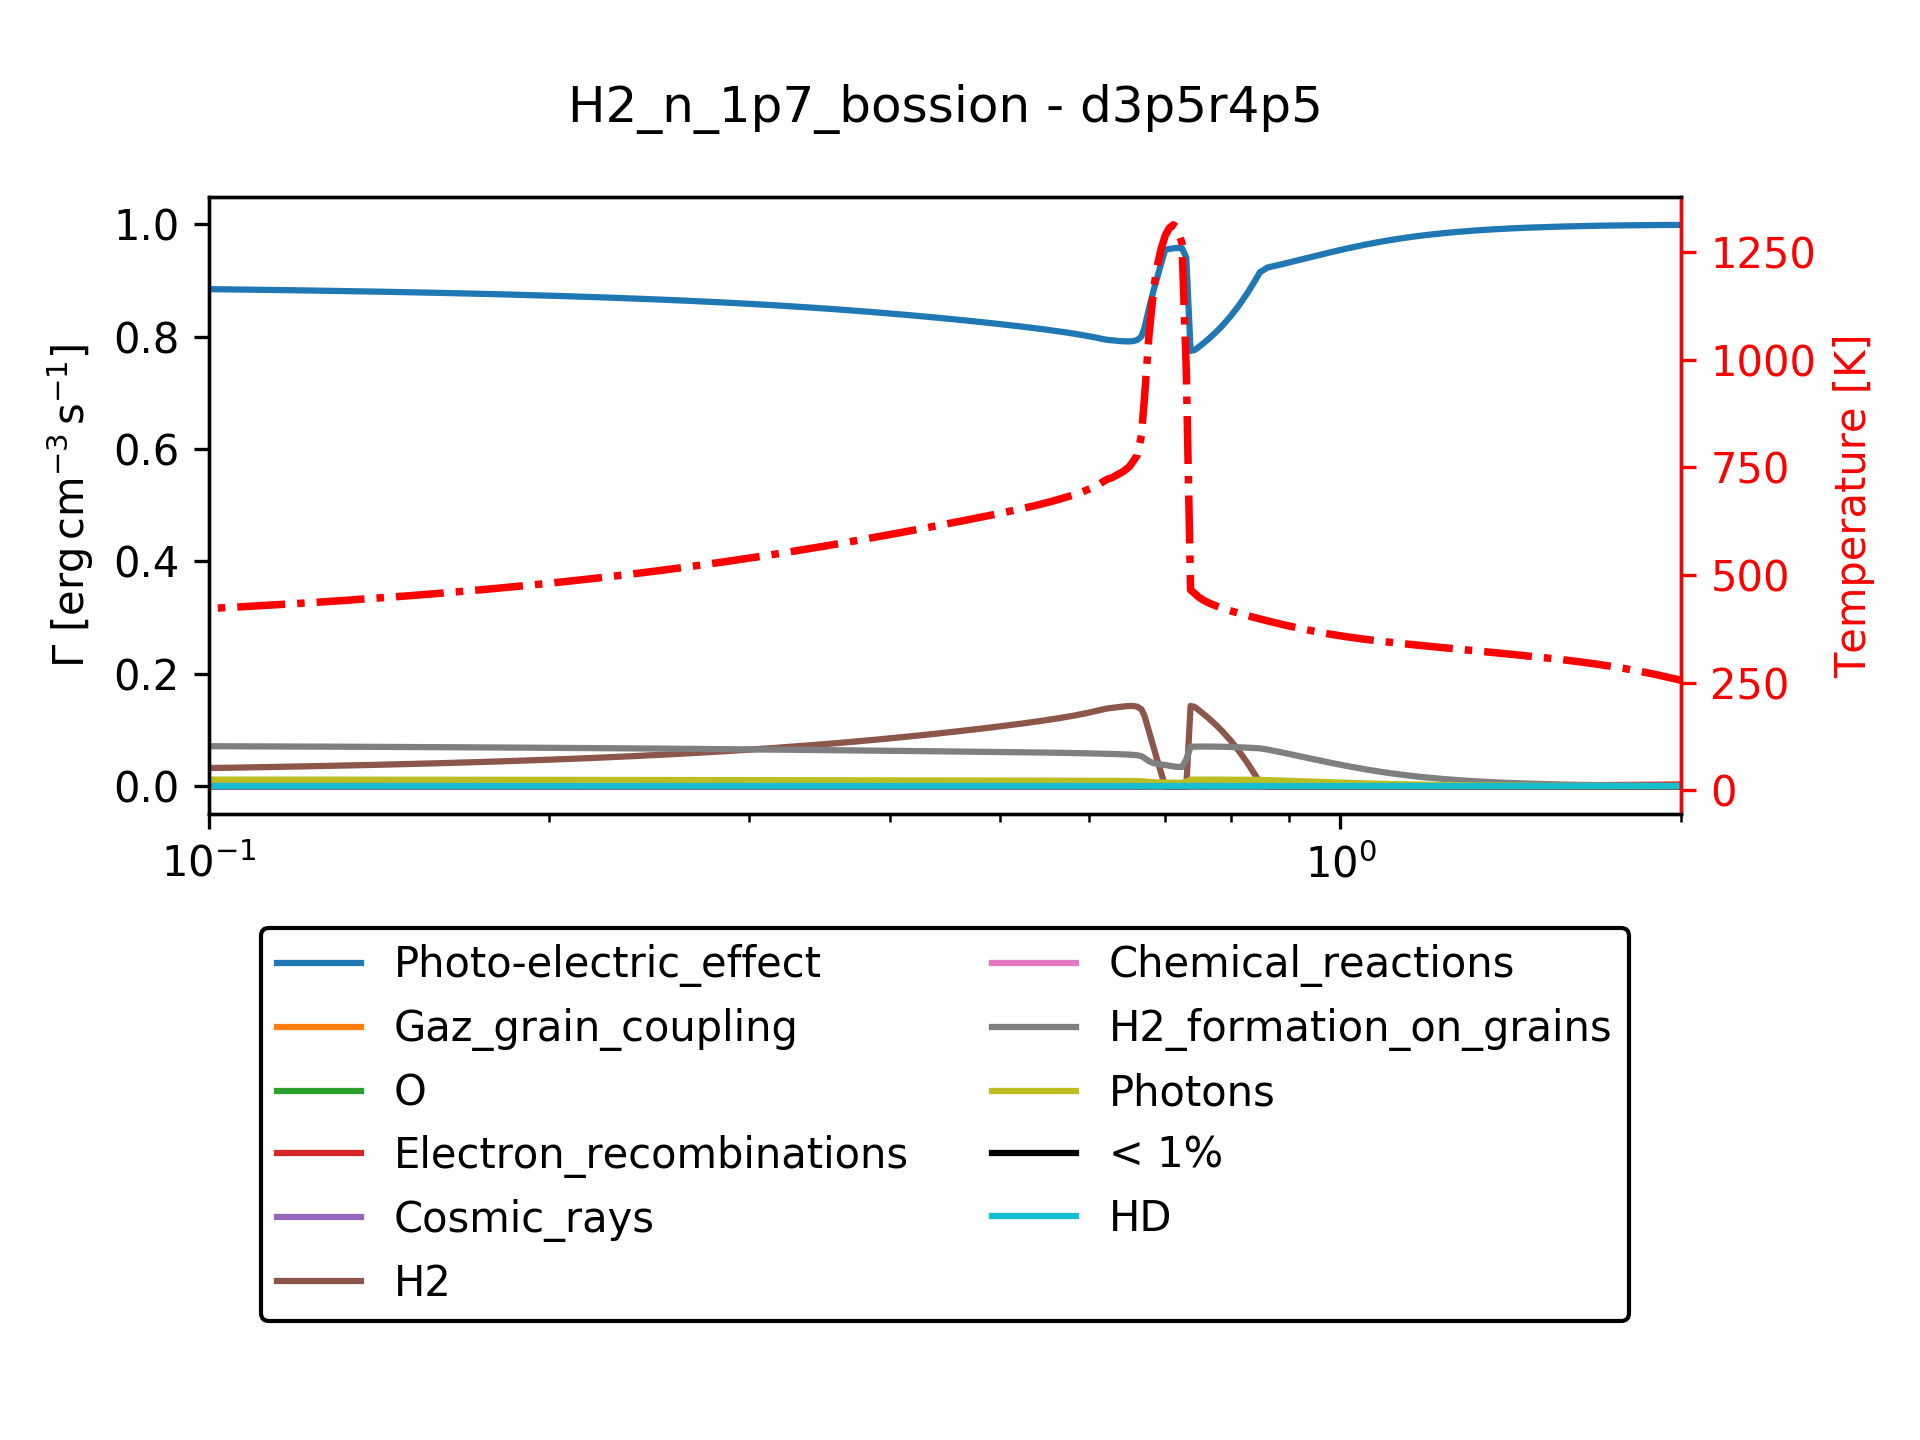
\includegraphics[trim = {0 0 0 1cm},clip,width=1\textwidth]{figure/H2/rec_elec/H2_n_1p7_bossion_d3p5r4p5hc_rheat.png}
%         \caption{Avec les nouveaux taux de collisions}
%     \end{subfigure}
%     ~ 
%     \begin{subfigure}[t]{0.49\textwidth} % "0.49" donne ici la largeur de l'image
%         \centering 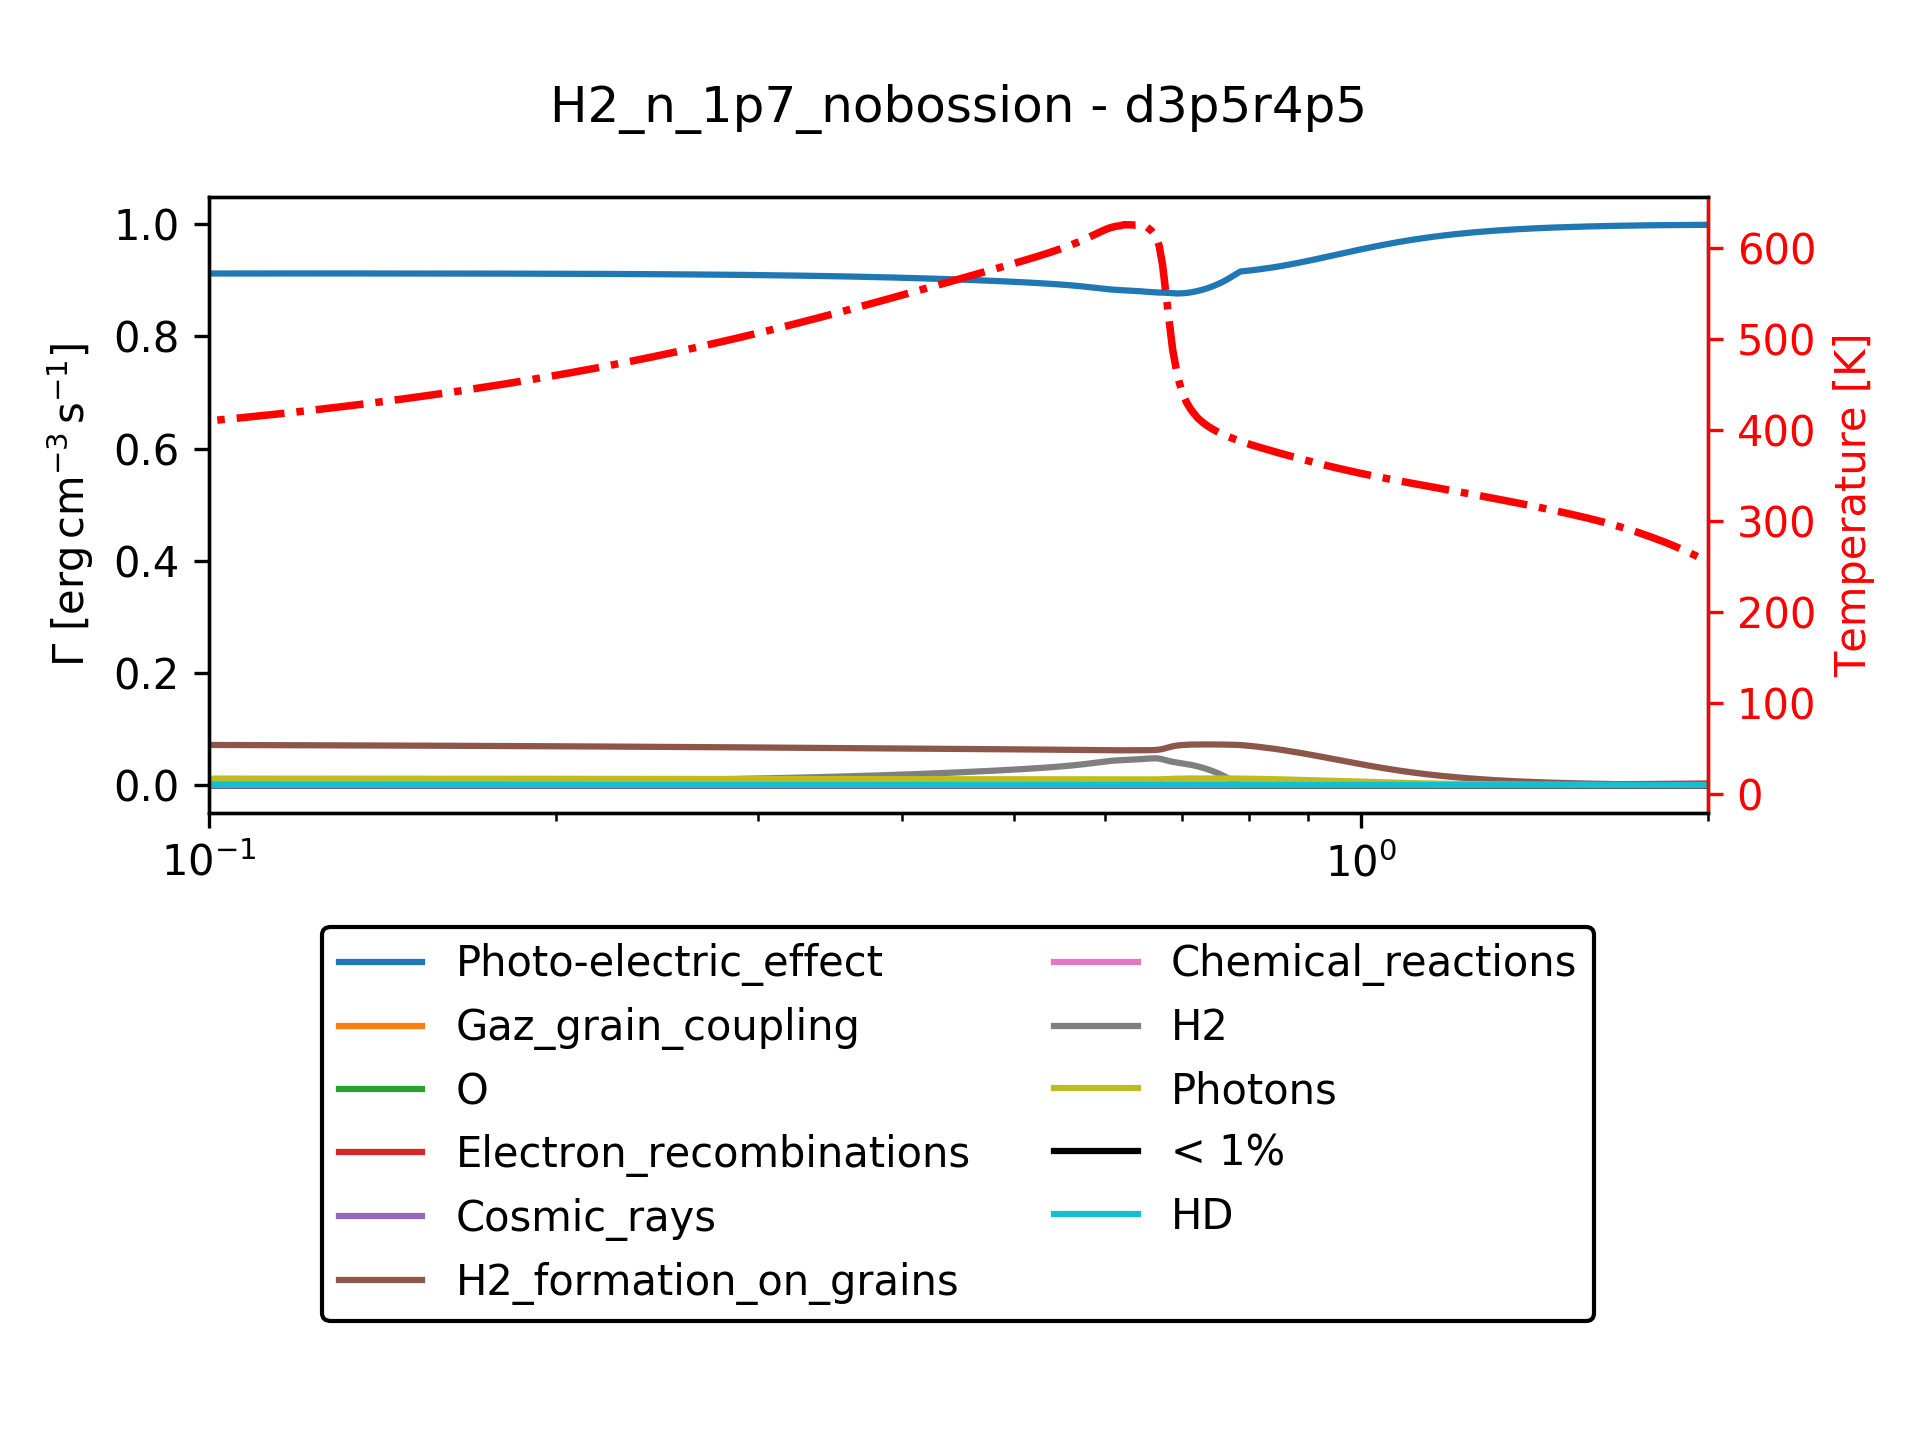
\includegraphics[trim = {0 0 0 1cm},clip,width=1\textwidth]{figure/H2/rec_elec/H2_n_1p7_nobossion_d3p5r4p5hc_rheat.png}
%         \caption{Sans les nouveaux taux de collisions}
%     \end{subfigure}
%     \caption{Taux de chauffage (en relatif) en fonction de l'extinction. Dans les deux situations le chauffage par effet photo-électrique est le phénomène dominant pendant l'irrégularité tandis que le chauffage par $\mathrm{H}_2$ devient refroidisseur. Cet effet est accentué si l'on prend en compte les nouveaux taux de collisions.}
%     \label{fig:H2:recomb:profilH}
% \end{figure}

% On a tracé une figure comparant la température, la densité de molécules $\mathrm{H}_2$ et la densité d'électrons à l'entrée du nuage moléculaire (\ref{fig:recomb:comp}). Ce pic abrupte est du à la prise en compte des taux de collisions. On observe aussi une monté (moindre) avec Janev et Glover sans les nouveaux taux (modèles densités constantes).

% \begin{figure}
%     \centering
%     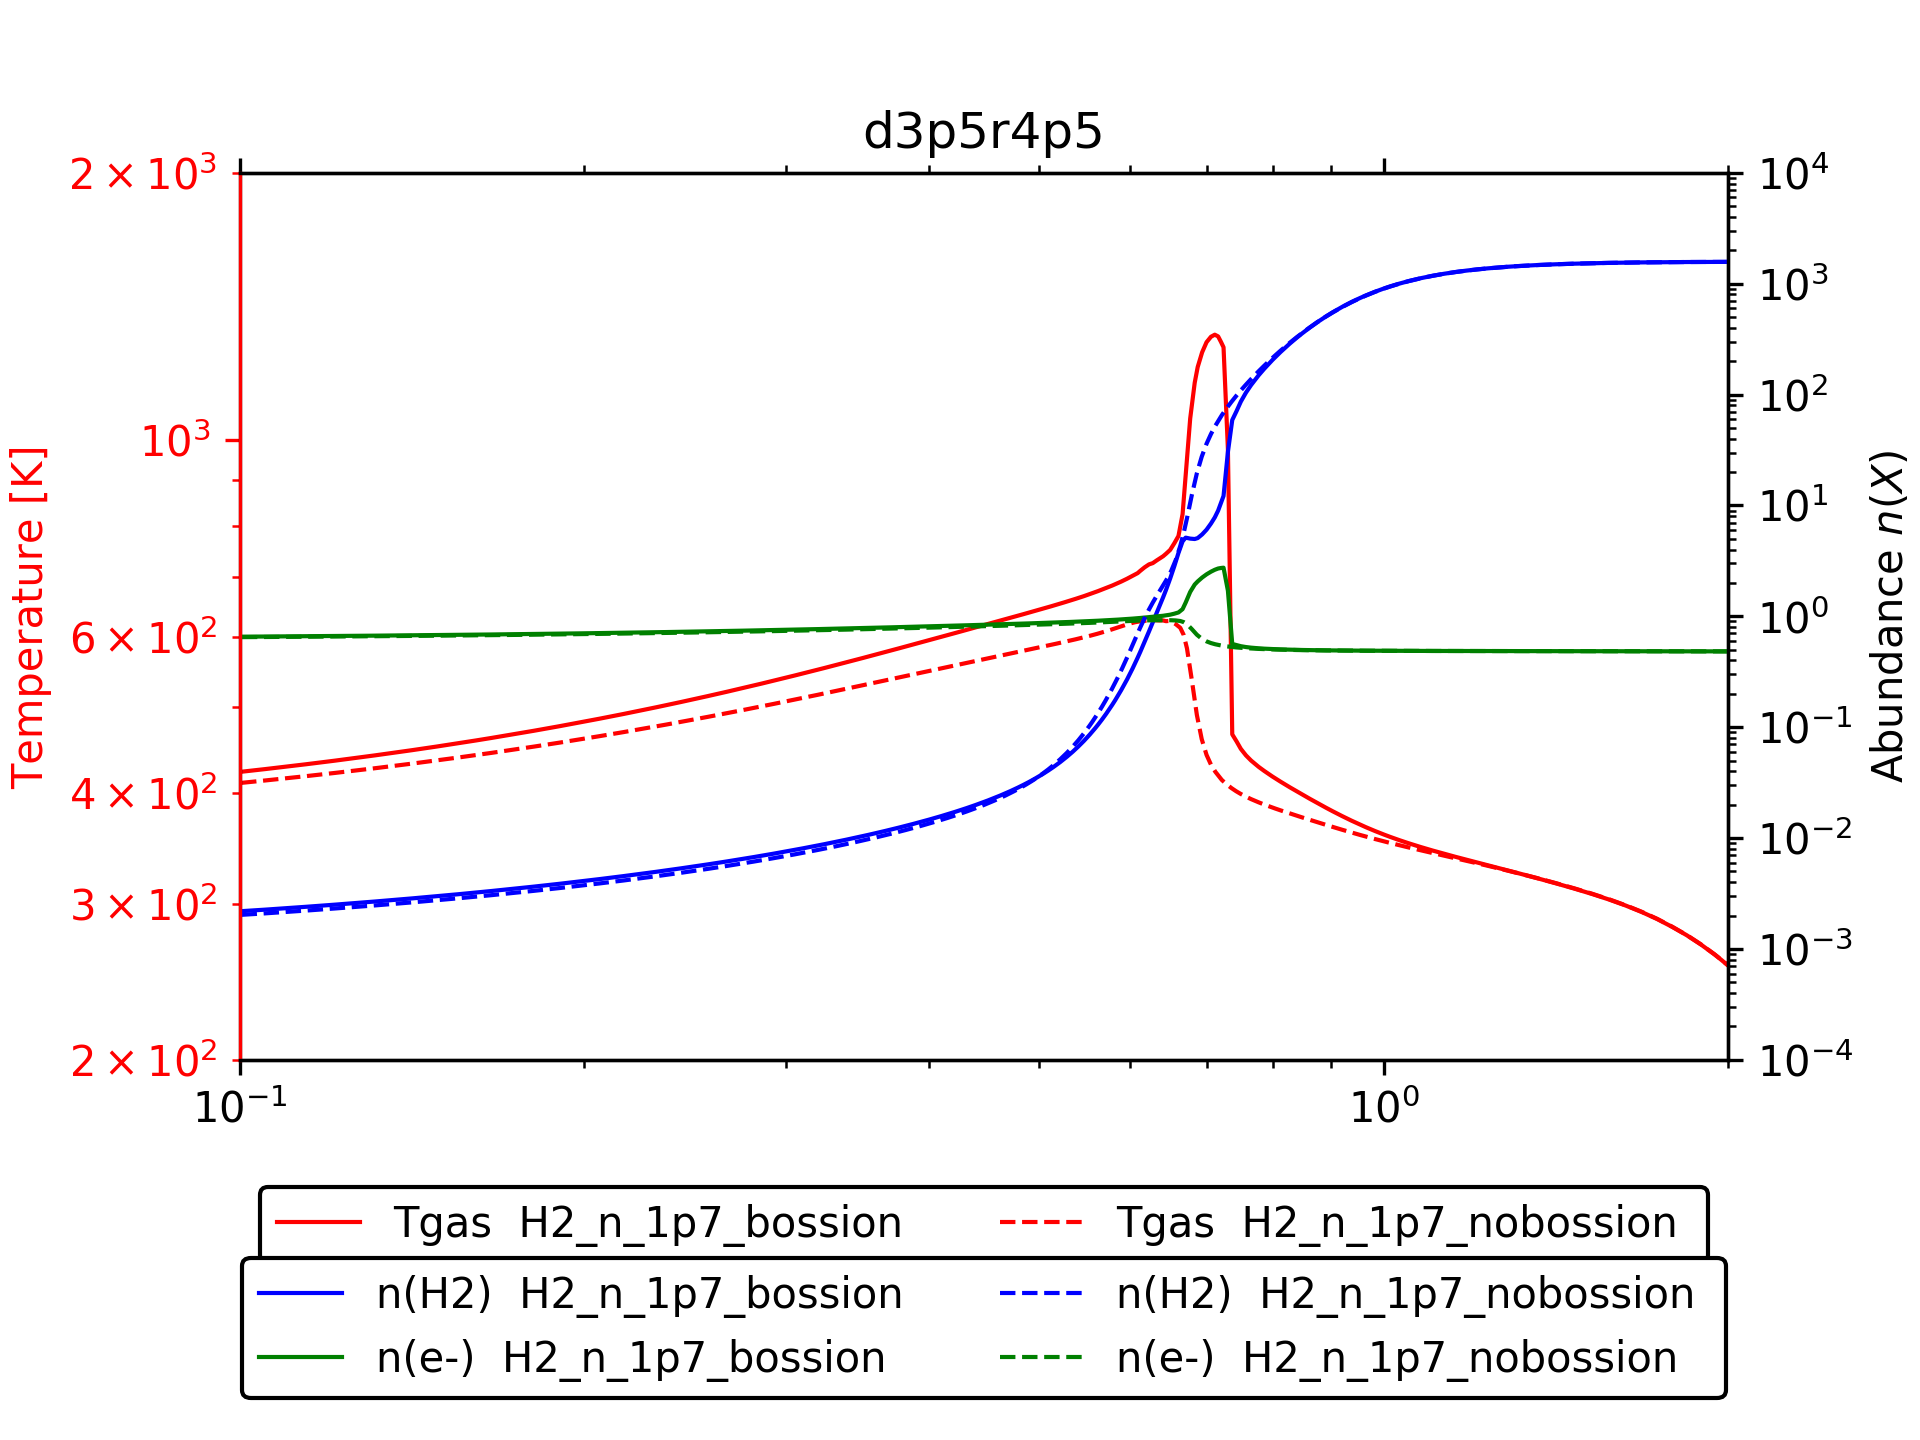
\includegraphics[trim = {0 0 0 0},clip,width=0.6\textwidth]{figure/H2/rec_elec/nT_H2_H2_n_1p7_bossion_H2_n_1p7_nobossion.png}
%     \caption{}
%     \label{fig:recomb:comp}
% \end{figure}